% (c) 2012 -2014 Claudio Carboncini - claudio.carboncini@gmail.com
% (c) 2012 -2014 Dimitrios Vrettos - d.vrettos@gmail.com
% (c) 2014 Daniele Zambelli - daniele.zambelli@gmail.com

\section{Esercizi}

\subsection{Esercizi dei singoli paragrafi}

% ------------------- Espressioni letterali ------------------

\subsubsection*{\numnameref{sec:esplett}}

\begin{inaccessibleblock}[Figura: TODO]
 \begin{figure}[b]
\begin{minipage}[t]{.45\textwidth}
 \centering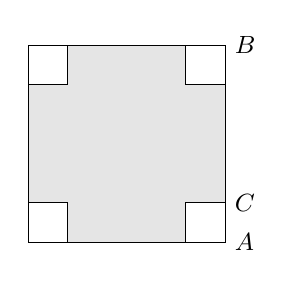
\begin{tikzpicture}[x=5mm, y=5mm,font=\small]
\definecolor{area}{gray}{0.9}
\draw [fill=area] (0,0) rectangle (5,5); 
\foreach \x in {0,4}{
\draw[fill=white] (\x,0) rectangle (\x+1,1);
\draw[fill=white] (\x,4) rectangle (\x+1,5);}
\node[right] at (5,0) {$A$};
\node [right] at (5,5) {$B$};
\node [right] at (5,1) {$C$};
\end{tikzpicture}
 \caption{Esercizio~\ref{ese:8.1}}\label{fig:8.1}
\end{minipage}
 \begin{minipage}[t]{.45\textwidth}
 \centering 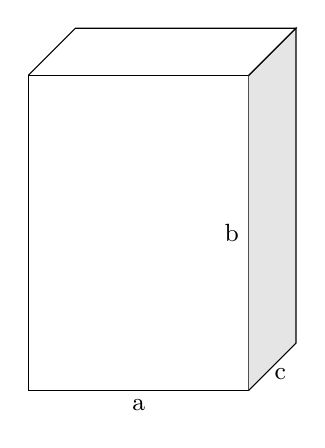
\begin{tikzpicture}[x=4mm, y=4mm,font=\small]
\definecolor{area}{gray}{0.9}
\draw(0,0) rectangle (7,10); 
\draw[fill=area, draw=black](7,0) -- (8.5,1.5)-- (8.5,11.5)--(7,10);
\draw(0,10) -- (1.5,11.5)-- (8.5,11.5)--(7,10);

\node[below] at (3.5,0) {a};
\node[left] at (7,5) {b};
\node[below] at (8,1) {c};
\end{tikzpicture}
 \caption{Esercizio~\ref{ese:8.10}}\label{fig:8.2}
\end{minipage}
\end{figure}
\end{inaccessibleblock}

\begin{multicols}{2}
\begin{esercizio}
\label{ese:8.1}
Esprimi con una formula l'area della superficie della zona colorata,
indicando con~$l$ la misura del lato~$AB$ e
con~$b$ la misura di~$AC$

\emph{Svolgimento}: l'area del quadrato è \ldots\ldots,
l'area di ciascuno dei quadratini bianchi è \ldots\ldots. 
Pertanto l'area della superficie in
grigio è \ldots\ldots
\end{esercizio}

\begin{esercizio}
\label{ese:8.2}
Scrivi l'espressione algebrica letterale relativa alla frase ``eleva al 
quadrato la differenza tra il cubo di un numero e il doppio del suo quadrato''.

\emph{Svolgimento}: detto~$a$ il numero generico, il cubo di~$a$ si indica 
con \ldots, il doppio quadrato di~$a$ si indica con \ldots e infine
il quadrato della differenza sarà: \ldots
\end{esercizio}

\begin{esercizio}
\label{ese:8.3}
Traduci in parole della lingua italiana il seguente schema di 
calcolo:~$(a-b)^{3}$

\emph{Svolgimento}: ``Eleva al \ldots\ldots la differenza tra \ldots\ldots''
\end{esercizio}

\begin{esercizio}
 \label{ese:8.4}
Individua tra le espressioni letterali sottostanti, quelle scritte 
correttamente:
\begin{enumeratea}
\spazielenx
 \item $b\cdot {\frac{4}{5}}+\left(3-\frac{7}{2}\right)\cdot a-a$
 \item $a\cdot +2-b^{4}$
 \item $x\cdot (a-b)^{2}+(x-3)$
 \item $x^{y}-a:2$
 \item $-a+4b+c$
 \item $\frac{a\cdot 1}{2}-\frac{a}{2}$
\end{enumeratea}
\end{esercizio}
\end{multicols}

\begin{esercizio}
\label{ese:8.5}
 Collega con una freccia la proprietà dell'operazione con la sua scrittura 
 attraverso lettere:
 \begin{multicols}{2}
 \noindent
 Commutativa dell'addizione\\
 Associativa della moltiplicazione\\
 Distributiva prodotto rispetto alla somma\\
 $a\cdot (x+y)=a\cdot x+a\cdot y$\\
 $\left(a\cdot b\right)\cdot c=a\cdot \left(b\cdot c\right)$\\
 ${a+b=b+a}$
 \end{multicols}
\end{esercizio}

\begin{esercizio}
\label{ese:8.6}
Esprimere con le lettere la proprietà commutativa della moltiplicazione

\emph{Svolgimento}: ``considerati~$a$ e~$b$ due numeri qualsiasi, la proprietà 
commutativa si esprime per mezzo dell'espressione \ldots\ldots; 
cioè \ldots\ldots\ldots''
\end{esercizio}

\begin{multicols}{2}
\begin{esercizio}
\label{ese:8.7}
Scrivi la formula che ci permette di calcolare l'area di un trapezio avente 
base maggiore~$B=5\unit{cm}$, base minore~$b=2\unit{cm}$ e 
altezza~$h=4\unit{cm}$
\end{esercizio}

\begin{esercizio}
\label{ese:8.8}
Scrivi la formula che permette di calcolare il lato di un quadrato di 
perimetro~$l$
\end{esercizio}

\begin{esercizio}
\label{ese:8.9}
Determina l'altezza~$h$ relativa all'ipotenusa~$BC$ del triangolo 
rettangolo~$ABC$

Caso \emph{numerico}:~$\overline{AB}=8\unit{m}$, $\overline{AC}=15\unit{m}.$

Caso \emph{generale}: Indica con~$x$ e~$y$ le misure dei cateti, e determina 
la formula per calcolare la misura di~$h_i$
\end{esercizio}

\begin{esercizio}
\label{ese:8.10}
Il volume della scatola (figura~\ref{fig:8.2}) avente le dimensioni 
di~$7\unit{cm}$, $10\unit{cm}$, $2\unit{cm}$ è~$\ldots$

Generalizza la questione indicando con~$a$, $b$, $c$ la misura delle sue 
dimensioni \ldots\ldots

Se raddoppiamo ciascuna dimensione allora il volume diventa
 \begin{enumeratea}
 \item $2\cdot a\cdot b\cdot c$
 \item $a^{2}\cdot b^{2}\cdot c^{2}$
 \item $6\cdot a\cdot b\cdot c$
 \item $8\cdot a\cdot b\cdot c$
 \end{enumeratea}
\end{esercizio}

% \begin{esercizio}[\Ast]
% \label{ese:8.11}
% Scrivi sotto forma di espressioni letterali le seguenti frasi:
%  \begin{enumeratea}
%  \item moltiplica~$a$ per l'inverso di~$a$
%  \item sottrai ad~$a$ l'inverso di~$b$
%  \item sottrai il doppio di~$a$ al cubo di~$a$
%  \end{enumeratea}
% \end{esercizio}

\begin{esercizio}
\label{ese:8.12}
Scrivi sotto forma di espressioni letterali le seguenti frasi:
 \begin{enumeratea}
 \item moltiplica~$a$ per l'opposto del cubo di~$a$:
 \item somma al triplo di~$a$ il doppio quadrato di~$b$
 \item moltiplica l'inverso di~$b$ per il quadrato dell'inverso di~$a$
 \item somma al cubo di~$a$ il quadrato della somma di~$a$ e~$b$
 \item dividi il quadrato di~$a$ per il triplo cubo di~$b$
 \item moltiplica il quadrato di~$b$ per l'inverso del cubo di~$a$
 \item il cubo di un numero, aumentato di~2, è uguale al quadrato della 
   differenza tra lo stesso numero e uno;
 \item il reciproco della somma dei quadrati di~$a$ e di~$b$
 \item il cubo della differenza tra~1 e il cubo di~$a$
 \item la somma dei quadrati di~$a$ e di~$b$ per il quadrato della 
   differenza tra~$a$ e~$b$
 \end{enumeratea}
\end{esercizio}
\end{multicols}

\subsubsection*{\numnameref{subsec:valnum}}

\begin{esercizio}
\label{ese:8.13}
Consideriamo l'espressione letterale~$E=-3\cdot a+2\cdot (-a+1)$

Osserviamo che vi compare una sola variabile, la lettera~$a$ supponiamo 
che~$E$ rappresenti uno schema di calcolo tra numeri interi relativi. 
Determiniamo il valore dell'espressione per alcuni valori della variabile:
\begin{align*}
a &=-2 \rightarrow \quad E =-3\cdot (-2)+2\cdot (-(-2)+1) =6+2\cdot (2+1) =6+6 
=12 \\
a &=+1 \rightarrow \quad E =-3\cdot (1)+2\cdot(-(1)+1) =-3+2\cdot (-1+1) =-3+0 
=-3 \\
a &=-1\ \rightarrow \quad E =-3\cdot (\ldots)+2\cdot (\ldots +1) =\ldots \ldots 
\ldots
\end{align*}

Completa la seguente tabella.

 \begin{tabular*}{.9\textwidth}{@{\extracolsep{\fill}}*{9}{c}}
 \toprule
 $a$ & $-2$ & $1$ & $-1$ & $0,1$ & $\dfrac{4}{5}$ & $-\dfrac{7}{5}$ & $-11$ 
&$0$\vspace{1.05ex}\\
 \midrule
 $E=-3a+2(-a+1)$& $12$ & $-3$ & & & & & &\\
 \bottomrule
 \end{tabular*}
\end{esercizio}

% \begin{esercizio}[\Ast]
% \label{ese:8.14}
% Calcola il valore dell'espressione letterale 
% $E=\frac{3}{7}\cdot a\cdot b-\frac{1}{2}\cdot (a-b)+a-b$ le cui 
% variabili~$a$, $b$ rappresentano numeri razionali, per i valori assegnati 
% nella tabella sottostante.
% 
% \emph{Svolgimento}: se vogliamo calcolare il valore dell'espressione 
% letterale dobbiamo scegliere due numeri razionali, uno da
% assegnare alla variabile~$a$, l'altro alla variabile~$b$
% 
% \begin{tabular*}{.9\textwidth}{@{\extracolsep{\fill}}*{5}{c}}
%  \toprule
%  $a$ & $3$ & $0$ & $2$ & $-{2}$\vspace{1.05ex}\\
%  $b$ & $-3$ & $-\dfrac{1}{2}$ & $0$ & $-\dfrac{3}{2}$ \\
%  \midrule
%  $E=\dfrac{3}{7} ab-\dfrac{1}{2}(a-b)+a-b$& & & &\\
%  \bottomrule
%  \end{tabular*}
% \end{esercizio}

\begin{esercizio}
\label{ese:8.15}
Calcolare il valore numerico 
dell'espressione:~$\dfrac{a}{a-3}+\dfrac{b}{3-b}$ per~$a = -1$, $b = 0$

\emph{Svolgimento}:~$\dfrac{-1}{-1-3}+\dfrac{0}{3-0}= \ldots\ldots$
\end{esercizio}

\begin{esercizio}
\label{ese:8.16}
Calcola il valore dell'espressione~$E=\dfrac{x-y}{3x}$ costruita con le 
variabili~$x$ e~$y$ che rappresentano numeri razionali. 
L'espressione letterale assegnata traduce il seguente schema di calcolo:
``la divisione tra la differenza di due numeri e il triplo del primo numero''. 
Completa la seguente tabella:

 \begin{tabular*}{.9\textwidth}{@{\extracolsep{\fill}}*{7}{c}}
 \toprule
 $x$ & $\dfrac{3}{4}$ & $\dfrac{19}{3}$ & $\dfrac{3}{4}$ & $-4$ & $\ldots$ & 
$\ldots$ \vspace{1.05ex}\\
 $y$ & $-2$ & $0$ & $0$ & $-2$ & $\ldots$ & $\ldots$ \\
 \midrule
 $E=\dfrac{x-y}{3x}$& & & & & &\\
 \bottomrule
 \end{tabular*}

Ti sarai accorto che in alcune caselle compare lo stesso valore per~$E$: 
perché secondo te succede questo fatto?

Vi sono, secondo te, altre coppie che fanno assumere ad~$E$ quello stesso 
valore?

\end{esercizio}

% \begin{esercizio}[\Ast]
% \label{ese:8.17}
% Scrivi con una frase le seguenti espressioni
% \begin{multicols}{2}
%  \begin{enumeratea}
% \spazielenx
%  \item $3a$
%  \item $\dfrac{2a}{3b^{2}}$
%  \end{enumeratea}
% \end{multicols}
% \end{esercizio}

\begin{esercizio}
\label{ese:8.18}
Scrivi con una frase le seguenti espressioni
\begin{multicols}{4}
 \begin{enumeratea}
\spazielenx
 \item $2b-5a$
 \item $a {\dfrac{1}{a}}$
 \item $(a+b)^{2}$
 \item $\dfrac{3x+y}{2x^{2}}$
 \end{enumeratea}
\end{multicols}
\end{esercizio}

% \newpage

\begin{esercizio}
\label{ese:8.19}
Completa la tabella sostituendo nella espressione della prima colonna i 
valori indicati.

 \begin{tabular*}{.93\textwidth}{l@{\extracolsep{\fill}}*{8}{c}}
 \toprule
 Espressione & $x=1$ & $x=-1$ & $x=0$ & $x=2$ & $x=\dfrac{1}{2}$ & 
$x=-\dfrac{1}{2}$ & $x=0,1$ & $x=\dfrac{1}{10}$\\
 \midrule
 $2x+1$ & & & & & & & &\\
 $-(3x-2)$ & & & & & & & &\\
 $x^{2}+2x+2$ & & & & & & & &\\
 $x^{2}-x$ & & & & & & & &\\
 $-x^{2}+x-1$ & & & & & & & &\\
 $x^{3}-1$ & & & & & & & &\\
 $x^{3}+3x^{2}$ & & & & & & & &\\
 $-x^{3}+x^{2}-x$ & & & & & & & &\\
 $-(x+1)^{2}$ & & & & & & & &\\
 \bottomrule
 \end{tabular*}
\end{esercizio}

\begin{esercizio}
\label{ese:8.20}
Calcola il valore numerico delle seguenti espressioni algebriche:
 \begin{enumeratea}
\spazielenx
 \item $3x^{2}-\dfrac{1}{4}x^{2}\quad$ per~$x=\dfrac{1}{2}\quad$ 
\emph{Svolgimento}:~$3\cdot \left(\dfrac{1}{2}\right)^{2}-\dfrac{1}{4}\cdot 
\left(\dfrac{1}{2}\right)^{2}=\ldots \ldots \ldots =\dfrac{11}{16}$
 \item $5a^{2}b\quad$ per~$a=-{\dfrac{1}{2}}$, $b=\dfrac{3}{5}\quad$ 
\emph{Svolgimento}:~$5\cdot \left(-{\dfrac{1}{2}}\right)^{2}\cdot 
\left(\dfrac{3}{5}\right)=\ldots \ldots \ldots \ldots $
 \item $\dfrac{3}{2}\cdot a^{2}+\dfrac{1}{2}a-1\quad$ per~$a=0$, per~$a=-1$ 
e~$a=2$
 \item $2\cdot x^{5}-8\cdot x^{4}+3\cdot x^{3}+2\cdot x^{2}-7\cdot x+8\quad$ 
per~$x=+1$ e~$x=-1$
 \end{enumeratea}
\end{esercizio}

\begin{esercizio}
\label{ese:8.21}
Calcola il valore numerico delle seguenti espressioni algebriche:
 \begin{enumeratea}
\spazielenx
 \item $(x-1)\cdot (x-2)\cdot (x+3)\quad$ per~$x=0$, $x= -1$ e~$x= 2$
 \item $x^{2}+2x+1\quad$ per~$x=0$, $x= -1$ e~$x= 1$
 \item $-a^{2}\cdot b\cdot c^{3}\quad$ per~$a=1$, $b=-1$, $c=-2$ e~$a=-1$, 
$b=\dfrac{9}{16}$, $c=\dfrac{4}{3}$
 \item $-{\dfrac{3}{2}}a+2b^{2}+11\quad$ per~$a=-20$, $b=-{\dfrac{1}{2}}$ 
e~$a=\dfrac{2}{3}$, $b=0$
 \item $-a^{2}+\dfrac{1}{a}-3\cdot a^{3}\quad$ per~$a=\dfrac{1}{3}$, $a=-1$ 
e~$a=+1$
 \end{enumeratea}
\end{esercizio}

% \begin{esercizio}[\Ast]
% \label{ese:8.22}
% Calcola il valore numerico delle seguenti espressioni algebriche:
%  \begin{enumeratea}
% \spazielenx
%  \item $4a+a^{3}\quad$ per~$a=2$ e~$a=1$ \hfill[2; 5]
%  \item $2a+5a^{2}\quad$ per~$a=-1$ e~$a=0$ \hfill[3; 0]
%  \item $3x+2y^{2}(xy)\quad$ 
%   per~$x=1$, $y=-{\dfrac{1}{2}}$ e~$x=\dfrac{1}{3}$, $y=-1$ 
\hfill[$\frac{11}{4}$]
%  \item $a^{2}-b^{-1}+ab\quad$ 
%   per~$a=1$, $b=\dfrac{1}{2}$ e~$a=0$, $b=-1$ \hfill[$-\frac{1}{2}$]
%  \item $3a^{2}b-7ab+a\quad$ per~$a=1$, $b=3$ e~$a=-1$, $b=-3$ \hfill[-11]
%  \end{enumeratea}
% \end{esercizio}

% \newpage

\begin{esercizio}[\Ast]
\label{ese:8.23}
Calcola il valore numerico delle seguenti espressioni algebriche:
 \begin{enumeratea}
\spazielenx
 \item $3xy-2x^{2}+3y^{2}\quad$ 
 per~$x=\dfrac{1}{2}$, $y=2$ e~$x=2$, $y=\dfrac{1}{2}$ \hfill[$\frac{29}{2}$]
 \item $\dfrac{2}{3}a\left(a^2-b^2 \right) \quad$ 
 per~$a=-3$, $b=-1$ e~$a=\dfrac{1}{3}$, $b=0$ \hfill[$-16$]
 \item $\dfrac{xy}{x}+3xy^{3}\quad$ 
 per~$x=2$, $y=-1$ e~$x=-2$, $y=+1$ \hfill[$-7$]
 \item $\dfrac{1}{2}\dfrac{(a+b)^{2}}{a^{2}b^{2}}+2a+3b\quad$ 
 per~$a=\dfrac{1}{4}$, $b=-2$ e $a=\dfrac{1}{2}$,$b=-{\dfrac{1}{2}}$ 
\hfill[$\frac{5}{8}$]
 \item $3x^{3}+2xy\left(\dfrac{x^{2}}{y}\right)+2y^{2}\quad$ 
 per~$x=-2$, $y=\dfrac{3}{4}$ e~$x=-1$, $y=-1$ \hfill[$\frac{311}{8}$]
 \end{enumeratea}
\end{esercizio}

% \begin{esercizio}[\Ast]
% \label{ese:8.24}
% Calcola il valore numerico delle seguenti espressioni algebriche:
%  \begin{enumeratea}
% \spazielenx
%  \item $\dfrac{4a-7b}{(2a+3b)^{3}}\cdot ab^{3}\quad$ 
%  per~$a=-{\dfrac{1}{2}}$, $b=1$ e~$a=-{\dfrac{1}{4}}$, $b=\dfrac{2}{3}$ 
% \hfill[$\frac{9}{16}$]
%  \item $\dfrac{4x^{2}-5xy+3y}{6x+y^{2}}\quad$ 
%  per~$x=-1$, $y=2$ e~$x=0$, $y=-2$ \hfill[-10]
%  \item $\dfrac{x}{x+3}+y^{2}-\dfrac{xy-3x+y}{(\mathit{xy})^{2}}\quad$ 
%  per~$x=3$, $y=\dfrac{1}{3}$ e~$x=1$, $y=-1$ \hfill[$\frac{149}{18}$]
%  \item $\dfrac{(4a-2b)\cdot {2a^{2}}}{3b^{3}}\cdot 
% {\dfrac{3}{4}}ab+a^{3}\quad$ 
%  per~$a=1$, $b=-1$ e~$a=0$, $b=-3$ \hfill[4]
%  \end{enumeratea}
% \end{esercizio}

\subsubsection*{\numnameref{subsec:condes}}

\begin{esercizio}
 \label{ese:8.25}
Se~$E=-{\dfrac{x-2}{2}x^{2}}$ completa la tabella:
\begin{center}
\begin{tabular*}{.4\textwidth}{l@{\extracolsep{\fill}}*{4}{c}}
\toprule
$x$ & 2 & 0 & $\dfrac{3}{4}$ & $-{\dfrac{5}{8}}$\\
E & & & & \\
\bottomrule
\end{tabular*}
\end{center}
\end{esercizio}

\begin{esercizio}
 \label{ese:8.26}
Calcola il valore numerico dell'espressione:~$\dfrac{3x-1}{x}$ per~$x = 0$

\emph{Svolgimento}: Sostituendo alla~$x$ il valore assegnato si ha una
divisione per \ldots e quindi \dotfill
\end{esercizio}

\begin{esercizio}[\Ast]
 \label{ese:8.27}
Sostituendo alle lettere i numeri, a fianco indicati, stabilisci se le
seguenti espressioni hanno significato:
\TabPositions{8cm}
\begin{enumeratea}
\item $\dfrac{x+3}{x}$\quad per~$x=0.$ \tab\boxSi\quad\boxNo
\item $\dfrac{x^{2}+y}{x}$\quad per~$x=3, y=0.$ \tab\boxSi\quad\boxNo
\item $\dfrac{(a+b)^{2}}{(a-b)^{2}}$\quad per~$a=1, b=1$ \tab\boxSi\quad\boxNo
\item $\dfrac{5x^{2}+3y-xy}{(x^{2}+y)^{3}}$\quad per~$x=2, y=-2$ 
\tab\boxSi\quad\boxNo
\item $\dfrac{a^{3}+b+6a^{2}}{a^{2}+b^{2}+3ab-3a^{2}}$\quad per~$a=1, 
b=\dfrac{4}{3}$ \tab\boxSi\quad\boxNo
\end{enumeratea}
\end{esercizio}

\begin{esercizio}
 \label{ese:8.28}
 Sostituendo alle lettere numeri razionali
arbitrari, determina se le seguenti uguaglianze tra formule sono
vere o false
\TabPositions{8cm}
\begin{enumeratea}
 \item $a^{2}+b^{2}=(a+b)^{2}$ \tab\boxV\quad\boxF
 \item $(a-b)\cdot (a^{2}+a\cdot b+b^{2})=a^{3}-b^{3}$ \tab\boxV\quad\boxF
 \item $(5a-3b)\cdot (a+b)=5a^{2}+ab-3b^{2}$ \tab\boxV\quad\boxF
\end{enumeratea}
\end{esercizio}

\begin{esercizio}
 \label{ese:8.29}
 Se~$n$ è un qualunque numero naturale,
l'espressione~$2\cdot n+1$ dà origine:
\begin{multicols}{2}
\boxA\quad ad un numero primo

\boxB\quad ad un numero dispari

\boxC\quad ad un quadrato perfetto

\boxD\quad ad un numero divisibile per~3
\end{multicols}
\end{esercizio}

\begin{esercizio}
 \label{ese:8.30}
 Quale formula rappresenta un multiplo di~5, qualunque sia il numero 
 naturale~$n$?
\begin{center}
 \boxA\quad~$5+n$ \quad\boxB\quad~$n^{5}$ \quad\boxC\quad~$5\cdot n$ 
\quad\boxD\quad~$\dfrac{n}{5}$
\end{center}
\end{esercizio}

\begin{esercizio}
 \label{ese:8.31}
 La tabella mostra i valori assunti da~$y$ al variare di~$x$ 
 Quale delle seguenti è la relazione tra~$x$ e~$y$?

\begin{center}
\begin{tabular*}{.4\textwidth}{l@{\extracolsep{\fill}}*{4}{c}}
\toprule
$x$ & 1 & 2 & 3 & 4\\
$y$ & 0 & 3 & 8 & 15\\
\bottomrule
\end{tabular*}

 \vspace{1.10ex}\boxA\quad~$y=x+1$ \quad\boxB\quad~$y=x^{2}-1$ 
\quad\boxC\quad~$y=2x-1$ \quad\boxD\quad~$y=2x^{2}-1$
\end{center}
\end{esercizio}

\begin{esercizio}
 \label{ese:8.32}
 Verifica che sommando tre numeri dispari consecutivi si ottiene un
multiplo di~3. Utilizza terne di numeri dispari che cominciano per~3;
7; 11; 15; 21. Per esempio~$3+5+7= \ldots$ multiplo di? Vero. Continua tu.
\end{esercizio}

% \subsection{Risposte}
% 
% \begin{multicols}{2}
% \paragraph{\ref{ese:8.11}}
% a)~$a \cdot\frac{1}{a}$,\quad b)~$a-\frac{1}{b}$,\quad c)~$a^3-2a$
% \paragraph{\ref{ese:8.14}}
% $a=3$ $b=-3\rightarrow -\frac{6}{7}$,\quad~$a=0$ $b=-\frac{1}{2}\rightarrow 
% \frac{1}{4}$,\quad~$a=-\frac{3}{2}$ $b=-\frac{3}{2}\rightarrow -\frac{27}{28}$
% \paragraph{\ref{ese:8.17}}
% a)~ Il triplo di~$a$,\quad ~b)~Dividi il doppio di~$a$ per il triplo del 
% quadrato di~$b$
% \paragraph{\ref{ese:8.22}}
% a)~$a=2 \rightarrow~16$ $a=1 \rightarrow~5$, \quad b)~$a=-1 \rightarrow~3$ 
% $a=0 \rightarrow~0$,
% c)~$x=1$ $y=-\frac{1}{2} \rightarrow \frac{11}{4}$,\quad d)~$a=1$ 
% $b=\frac{1}{2}\rightarrow -\frac{1}{2}$, \quad e)~$a=1$ $b=3 \rightarrow -11$
% \paragraph{\ref{ese:8.23}}
% a)~$x=\frac{1}{2}$ $y=2 \rightarrow \frac{29}{2}$, \quad b)~$a=-3$ $b=-1 
% \rightarrow -16$, \quad c)~$x=2$,$y=-1 \rightarrow -7$,
% d)~$a=\frac{1}{4}$ $b=-2 \rightarrow \frac{5}{8}$,\quad e)~$x=-2$ 
% $y=\frac{3}{4} \rightarrow -\frac{311}8{}$,\quad
% \paragraph{\ref{ese:8.24}}
% a)~$a=-\frac{1}{2}$ $b=1 \rightarrow \frac{9}{16}$,
% b)~$x=-1$ $y=2 \rightarrow -10$,\quad c)~$x=3$ $y=\frac{1}{3} \rightarrow 
% \frac{149}{18}$,\quad d)~$a=1$ $b=-1 \rightarrow~4$
% \paragraph{\ref{ese:8.27}}
% a)~Non ha significato perché $\frac{4}{0}$ non è un numero.
% \end{multicols}

% ------------------- Monomi ------------------

%\subsubsection*{9.1 - L'insieme dei monomi}
\subsubsection*{\numnameref{subsec:09_monomi_definizioni}}

\begin{esercizio}
\label{ese:9.1}
Individua tra le espressioni letterali di seguito elencate, quelle che sono 
monomi.
\[E_{1}=35x^{2}+y^{2}; E_{2}=-4^{-1}ab^{4}c^{6}; E_{3}=\dfrac{4}{x}y^{2}; 
E_{4}=-{\frac{87}{2}}x^{2}z.\]

Per rispondere in modo corretto devo individuare quelle espressioni in
cui compare solamente la \dotfill; pertanto sono monomi \dotfill
\end{esercizio}

\begin{esercizio}
\label{ese:9.2}
Scrivi in forma normale i seguenti monomi:
\begin{multicols}{2}
 $\dfrac{4}{9}ab18c^{3}2^{-2}a^{3}b=\dfrac{\ldots }{\ldots }a^{\ldots}b^{\ldots 
}c^{\ldots };$

 $-x^{5}\dfrac{1}{9}y^{4}\big(-1+5\big)^{2}y^{7}=\dotfill~$
\end{multicols}
\end{esercizio}

\begin{esercizio}
\label{ese:9.3}
Nell'insieme
$M=\big\{-{\frac{34}{5}}a^{3}b, 3^{2}a^{2}b^{4}, \frac{1}{3}ab^{3}, a^{3}b, -a, 
7a^{2}b^{4}, -\frac{1}{3}ab^{3}, -89a^{3}b\big\}$,
determina i sottoinsiemi dei monomi simili; rappresenta con un diagramma di 
Venn.
\end{esercizio}

%\subsubsection*{9.2 - Valore di un monomio}
\subsubsection*{\numnameref{subsec:09_monomi_valore}}

\begin{esercizio}
\label{ese:9.4}
Calcola l'area di un triangolo che ha altezza~$h=2,5$ e base~$b=\frac{3}{4}$
\end{esercizio}

\begin{esercizio}
 \label{ese:9.5}
 Calcola il valore dei seguenti monomi in corrispondenza dei valori indicati per 
ciascuna lettera.

\begin{multicols}{2}
\begin{enumeratea}
 \item $-\frac{2}{9}xz$ per $ x=\frac{1}{2} $, $z=-1$
 \item $-\frac{8}{5}x^{2}y$ per $ x=-1 $, $y=+10$
 \item $-\frac{1}{2}a^{2}bc^3$ per $ a=-\frac{1}{2} $, $b=\frac{3}{2},c=-1$
 \item $\frac{7}{2}a^{3}x^{4}y^2$ per $ a=\frac{1}{2} $, $x=2$, $y=-\frac{1}{2}$
 \item $\frac{8}{3}abc^2$ per $ a=-3 $, $b=-\frac{1}{3},c=\frac{1}{2}$
\end{enumeratea}
\end{multicols}
\end{esercizio}


\begin{esercizio}
 \label{ese:9.6}
 Il grado complessivo di un monomio è:

\begin{enumeratea}
 \item l'esponente della prima variabile che compare nel monomio;
 \item la somma di tutti gli esponenti che compaiono sia ai fattori
numerici sia a quelli letterali;
 \item il prodotto degli esponenti delle variabili che compaiono nel monomio;
 \item la somma degli esponenti di tutte le variabili che vi compaiono.
\end{enumeratea}
\end{esercizio}


\begin{esercizio}
 \label{ese:9.7}
Due monomi sono simili se:

\begin{enumeratea}
 \item hanno lo stesso grado;
 \item hanno le stesse variabili;
 \item hanno lo stesso coefficiente;
 \item hanno le stesse variabili con rispettivamente gli stessi esponenti.
\end{enumeratea}
\end{esercizio}

\begin{esercizio}
 \label{ese:9.8}
Individua e sottolinea i monomi tra le seguenti espressioni letterali:
\[3+ab; -2a; -\frac{7}{3}ab^2; -(\frac{4}{3})^{3}; 
a^{2}bc\cdot{\frac{-2}{a^{3}}}; 4a^{-3}b^{2}c^{5}; -x; 8x^{4}-4x^{2}; 
-y\cdot(2x^{4}+6z); \frac{abc^{9}}{3+7^{-2}}\]
\end{esercizio}

\begin{esercizio}
 \label{ese:9.9}
Nel monomio~$m=-{\frac{5}{2}}a^{3}x^{2}y^{4}z^{8}$ distinguiamo: 
coefficiente~$=\ldots$,
parte letterale~$=\ldots$,
grado complessivo~$=\ldots$,
il grado della lettera~$x=\ldots$
\end{esercizio}

\begin{esercizio}
 \label{ese:9.10}
Motiva brevemente la verità o falsità delle seguenti proposizioni:
\TabPositions{8.5cm}
\begin{enumeratea}
 \item ``Se due monomi hanno ugual grado allora sono 
simili''\tab\boxV\quad\boxF\qquad perché\dotfill
 \item ``Se due monomi sono simili allora hanno lo stesso 
grado''\tab\boxV\quad\boxF\qquad perché\dotfill
\end{enumeratea}
\end{esercizio}

\begin{esercizio}
 \label{ese:9.11}
Quale diagramma di Venn rappresenta in modo corretto la seguente proposizione: 
<<alcune espressioni letterali non sono monomi>>.
$L$: insieme delle espressioni letterali, $M$: insieme dei monomi.
\begin{center}
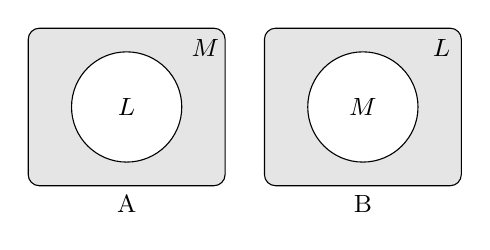
\begin{tikzpicture}[x=5mm, y=5mm,font=\small]
\definecolor{area}{gray}{0.9}
\draw [rounded corners, fill=area] (0,0) rectangle (5,4)  (4.5,3.5)node {$M$}; 
\draw[fill=white] (2.5,2) circle (1.4) node {$L$};
\node[below] at (2.5,0) {A};

\begin{scope}[xshift=30mm]
\draw [rounded corners, fill=area] (0,0) rectangle (5,4)  (4.5,3.5)node {$L$}; 
\draw[fill=white] (2.5,2) circle (1.4) node {$M$};
\node[below] at (2.5,0) {B};
\end{scope}
\end{tikzpicture}
\end{center}
\end{esercizio}

\begin{esercizio}
 \label{ese:9.12}
 Attribuisci il valore di verità alle seguenti proposizioni:
\TabPositions{11.5cm}
\begin{enumeratea}
\item Il valore del monomio~$-a$ è negativo per qualunque a diverso da 
zero.\tab\boxV\quad\boxF
\item Il valore del monomio~$-a^{2}$ è negativo per qualunque a diverso da 
zero.\tab\boxV\quad\boxF
\item Il monomio~$b^{6}$ è il cubo di~$b^{2}$\tab\boxV\quad\boxF
\item L'espressione~$ab^{-1}$ è un monomio.\tab\boxV\quad\boxF
\item Il valore del monomio ab è nullo per~$a = 1 e b =-1$\tab\boxV\quad\boxF
\end{enumeratea}
\end{esercizio}


%\subsubsection*{9.3 - Moltiplicazione di due monomi}
\subsubsection*{\numnameref{subsec:09_monomi_prodotto}}

\begin{esercizio}
 \label{ese:9.13}
Determina il prodotto dei seguenti monomi.
\begin{multicols}{2}
\begin{enumeratea}
\spazielenx
 \item $\big(-x^{2}y^{4}\big)\cdot \bigg(-{\dfrac{8}{5}}x^{2}y\bigg)$
 \item 
$\bigg(-{\dfrac{15}{28}}xy^{3}\bigg)\cdot\bigg(-\dfrac{7}{200}x^{2}y^{2}\bigg)$
 \item $\big(a^{5}b^{5}y^{2}\big)\cdot\bigg(-\dfrac{8}{5}a^{2}y^{2}b^{3}\bigg)$
 \item $2,5ab^{2}\cdot \bigg(-{\dfrac{1}{2}}a^{2}b\bigg)\cdot 1,5a$
 \item $\bigg(-{\dfrac{2}{9}}xz\bigg)\bigg(-{\dfrac{1}{4}}z^{3}\bigg)(27x)$
 \item $-8\bigg(\dfrac{1}{4}x\bigg)\bigg(\dfrac{4}{5}x^{3}a^{4}\bigg)$
 \item $5x^{3}y^{2}\cdot \bigg(-{\dfrac{1}{3}}x^{3}y^{2}\bigg)\cdot 
\bigg(-{\dfrac{1}{3}}\bigg)$
 \item $6ab\cdot \bigg(-{\dfrac{1}{3}}a^{2}\bigg)\cdot {\dfrac{1}{2}ab\cdot 
4a^{2}}$
%  \item $\bigg(\dfrac{7}{2}a^{3}x^{4}y^{2}\bigg)\cdot 
% \bigg(-{\dfrac{8}{21}}ax^{2}y\bigg)$
\end{enumeratea}
\end{multicols}
\end{esercizio}


\begin{esercizio}
 \label{ese:9.14}
Determina il prodotto dei seguenti monomi.
\begin{multicols}{3}
\begin{enumeratea}
\spazielenx
 \item $(-2xy)\cdot (+3ax)$
 \item $6a(-2ab)\big(-3a^{2}b^{2}\big)$
 \item $(-1)(-ab)$
 \item $1,5a^{2}b\cdot \bigg(-{\dfrac{2}{3}}a^{2}b\bigg)$
 \item $-{\dfrac{7}{5}}xy^{3}\bigg(-{\dfrac{10}{3}}xy^{2}z\bigg)$
 \item $-x\big(14x^{2}\big)$
\end{enumeratea}
\end{multicols}
\end{esercizio}

\begin{esercizio}
 \label{ese:9.15}
Determina il prodotto delle seguenti coppie di monomi.
\begin{multicols}{3}
\begin{enumeratea}
 \item $1,\overline{6}xa\big(1,2xy^{2}\big)$
 \item $\bigg(\dfrac{12}{7}m^{2}n^{3}\bigg)\bigg(-{\dfrac{7}{4}}mn\bigg)$
 \item $\bigg(-{\dfrac{5}{4}}ax^{2}\bigg)\bigg(\dfrac{3}{10}x^{3}y\bigg)$
 \item $12ab\bigg(-{\dfrac{1}{2}}a^{3}b^{3}\bigg)$
 \item $\bigg(-{\dfrac{15}{8}}at^{2}\bigg)\bigg(\dfrac{6}{5}t^{3}x\bigg)$
 \item $\bigg(\dfrac{12}{4}a^{2}n^{2}\bigg)\bigg(-{\dfrac{7}{4}}ax\bigg)$
\end{enumeratea}
\end{multicols}
\end{esercizio}


\begin{esercizio}
 \label{ese:9.16}
Sulla base degli esercizi precedenti puoi concludere che il grado del monomio 
prodotto è:

\begin{enumeratea}
 \item il prodotto dei gradi dei suoi fattori;
 \item la somma dei gradi dei suoi fattori;
 \item minore del grado di ciascuno dei suoi fattori;
 \item uguale al grado dei suoi fattori.
\end{enumeratea}
\end{esercizio}

%\subsubsection*{9.4 - Potenza di un monomio}
\subsubsection*{\numnameref{subsec:09_monomi_potenza}}

\begin{esercizio}
 \label{ese:9.17}
 Esegui le potenze indicate.
\begin{multicols}{2}
\begin{enumeratea}
\spazielenx
 \item $\bigg(-{\dfrac{3}{5}}abx^{3}y^{5}\bigg)^{3}=\dfrac{\ldots 
}{\ldots}a^{3}b^{3}x^{\ldots }y^{\ldots}$
 \item $\big(-a^{4}b^{2}\big)^{7}=\ldots$
 \item $\bigg(-3x^{3}y^{4}z\bigg)^{2}=9x^{6}y^{\ldots }z^{\ldots }$
 \item 
$\bigg(\dfrac{1}{2}a^{2}bc^{5}\bigg)^{4}=\dfrac{1}{\ldots}a^{\ldots}b^{\ldots}c^
{\ldots}$
 \item $\big(a^{3}b^{2}\big)^{8}=\ldots$
 \item $\big(-5ab^{2}c\big)^{3}=\ldots$
\end{enumeratea}
\end{multicols}
\end{esercizio}

\newpage %------------------------------------------------------------------

\begin{esercizio}
 \label{ese:9.18}
 Esegui le potenze indicate.
\begin{multicols}{3}
\begin{enumeratea}
\spazielenx
 \item $\big(+2ax^{3}y^{2}\big)^{2}$
 \item $\bigg(-{\dfrac{1}{2}}axy^{2}\bigg)^{3}$
 \item $\bigg(\dfrac{3}{4}x^{4}y\bigg)^{3}$
 \item $\bigg(\dfrac{2}{3}xy^{2}\bigg)^{3}$
 \item $\bigg(-{\dfrac{1}{2}}ab\bigg)^{4}$
 \item $\bigg(-{\dfrac{3}{2}}a^{5}\bigg)^{2}$
\end{enumeratea}
\end{multicols}
\end{esercizio}

\begin{esercizio}
 \label{ese:9.19}
 Esegui le operazioni indicate.
\begin{multicols}{2}
\begin{enumeratea}
\spazielenx
 \item $\bigg[\big(-rs^{2}t\big)^{2}\bigg]^{3}$
 \item $\Bigg[\bigg(-{\dfrac{1}{2}}x^{2}y^{3}\bigg)^{2}\Bigg]^{3}$
 \item $\Bigg[\bigg(-{\dfrac{3}{2}}a^{2}b^{3}\bigg)^{2}\Bigg]^{2}$
 \item $\big(-xy\big)^{2}\bigg(-{\dfrac{1}{2}}xy^{2}\bigg)^{3}$
 \item 
$-\bigg(\dfrac{3}{2}xy^{2}\bigg)^{0}\cdot\bigg(-{\dfrac{1}{6}}xy\bigg)^{2}$
 \item 
$-\bigg(-{\dfrac{1}{3}}x^{3}y^{2}\bigg)^{2}\cdot
\bigg(-{\dfrac{1}{3}}\bigg)^{-3}$
 \item $\bigg(\dfrac{2}{3}ab^{2}c\bigg)^{2}\cdot\big(-3ab^{3}\big)^{2}$
 \item 
$\Bigg[\bigg(-{\dfrac{1}{2}}a^{2}b\bigg)^{2}\cdot{\dfrac{2}{3}a^{2}b}\Bigg]^{2}$
%  \item $\bigg(\dfrac{2}{3}x\cdot{\dfrac{1}{6}}x\cdot 
% {\dfrac{1}{2}}x\bigg)^{2}\cdot\bigg(-{\dfrac{1}{6}}ab^{2}\bigg)^{2}$
\end{enumeratea}
\end{multicols}
\end{esercizio}

%\subsubsection*{9.5 - Divisione di due monomi}
\subsubsection*{\numnameref{subsec:09_monomi_quoziente}}

\begin{esercizio}
 \label{ese:9.21}
Esegui le divisioni indicate e poni le~$\CE$:
\begin{multicols}{2}
\begin{enumeratea}
\spazielenx
 \item $15b^{8}:\bigg(-{\dfrac{40}{3}}b^{3}\bigg)$
 \item 
$\bigg(-{\dfrac{13}{72}}x^{2}y^{5}z^{3}\bigg):\bigg(-{\dfrac{26}{27}}xyz\bigg)$
 \item $(-a^{7}):(8a^{7})$
 \item $\bigg(\dfrac{1}{2}a^{3}\bigg):(-4a^{5})$
 \item $\bigg(-{\dfrac{12}{2}}a^{7}b^{5}c^{2}\bigg):(-18ab^{4}c)$
 \item $(-34x^{5}y^{2}):(-2yz^{3})$
\end{enumeratea}
\end{multicols}
\end{esercizio}

\begin{esercizio}
 \label{ese:9.22}
Esegui le divisioni indicate e poni le~$\CE$:
\begin{multicols}{2}
\begin{enumeratea}
 \item $21a^{3}x^{4}b^{2}:7ax^{2}b$
 \item $a^{6}:20a^{2}$
 \item $20ax^{4}y:2xy$
 \item $-72a^{4}b^{2}y^{2}:(-3ab^{2})$
\end{enumeratea}
\end{multicols}
\end{esercizio}

\begin{esercizio}
 \label{ese:9.23}
Esegui le operazioni indicate e poni le~$\CE$:
\begin{multicols}{2}
\begin{enumeratea}
 \item $48a^{5}bx:a^{2}b$
 \item 
$\Bigg[-\bigg(-{\dfrac{1}{3}}x^{3}y^{2}\bigg)^{2}:\bigg(-{\dfrac{1}{3}}
\bigg)\Bigg]^{2}:(x^{3}y^{2})^{2}$
 \item 
$\Bigg[\dfrac{3}{5}x^{4}:\bigg(\dfrac{1}{3}x^{4}\bigg)\Bigg]\cdot\Bigg[x^{4}
:\bigg(\dfrac{4}{5}x^{4}\bigg)\Bigg]$
 \item $\bigg(\dfrac{2}{3}ab^{2}c\bigg)^{2}:(-3ab^{3})$
\end{enumeratea}
\end{multicols}
\end{esercizio}

%\subsubsection*{9.6 - Addizione di due monomi simili}
\subsubsection*{\numnameref{subsec:09_monomi_somma}}

\begin{esercizio}
 \label{ese:9.24}
Determina la somma dei monomi 
simili~$8a^{2}b+(-{\frac{2}{3}})a^{2}b+\frac{1}{6}a^{2}b$

La somma è un monomio \ldots\ldots\ldots agli
addendi; il suo coefficiente è dato da
$8-\frac{2}{3}+\frac{1}{6}=\ldots $, la parte letterale è~$\dotfill~$ Quindi la
somma è~$\dotfill$
\end{esercizio}

\begin{esercizio}
 \label{ese:9.25}
Determina la somma~$S=2a-3ab-a+17ab+41a$

I monomi addendi non sono tra loro simili, modifico la scrittura
dell'operazione applicando le proprietà associativa e commutativa
in modo da affiancare i monomi simili:
\[
S=2a-3ab-a+17ab+41a=(\ldots\ldots\ldots)+(\ldots\ldots\ldots)=\ldots\ldots\ldots
\]
La somma ottenuta non è un \ldots\ldots\ldots\ldots\ldots
\end{esercizio}

\begin{esercizio}
 \label{ese:9.26}
Esegui la somma algebrica dei seguenti monomi.
\begin{multicols}{3}
\begin{enumeratea}
 \item $6x+2x-3x$
 \item $-3a+2a-5a$
 \item $5a^{2}b-3a^{2}b$
 \item $a^{2}b^{2}-3a^{2}b^{2}$
 \item $2xy-3xy+xy$
 \item $2y^{2}-3y^{2}+7y^{2}-4y^{2}$
\end{enumeratea}
\end{multicols}
\end{esercizio}

\begin{esercizio}
 \label{ese:9.27}
Esegui la somma algebrica dei seguenti monomi.
\begin{multicols}{3}
\begin{enumeratea}
 \item $-2xy^{2}+xy^{2}$
 \item $-3ax-5ax$
 \item $5ab-2ab$
 \item $-3xy^{2}+3xy^{2}$
 \item $7xy^{3}-2xy^{3}$
 \item $+2xy^{2}-4xy^{2}$
\end{enumeratea}
\end{multicols}
\end{esercizio}

\begin{esercizio}
 \label{ese:9.28}
Esegui la somma algebrica dei seguenti monomi.
\begin{multicols}{2}
\begin{enumeratea}
 \item $\dfrac{1}{2}a^{2}-a^{2}$
 \item $+2xy^{2}-4xy^{2}+xy^{2}$
 \item $-5x^{2}+3x^{2}$
 \item $\dfrac{1}{2}a+2a$
 \item $5a^{2}b+2a^{2}b+a^{2}b-3a^{2}b-a^{2}b$
 \item $0,1x-5x-1,2x+3x$
\end{enumeratea}
\end{multicols}
\end{esercizio}

\begin{esercizio}
 \label{ese:9.29}
Esegui la somma algebrica dei seguenti monomi.
\begin{multicols}{2}
\begin{enumeratea}
\spazielenx
 \item $\dfrac{1}{4}a^{3}b^{2}-\dfrac{1}{2}a^{3}b^{2}$
 \item $\dfrac{2}{3}x-\dfrac{2}{5}x-2x+\dfrac{3}{10}x$
 \item 
$\dfrac{2}{5}ab-\dfrac{1}{2}ab+\dfrac{27}{2}ab-\dfrac{1}{10}ab-\dfrac{5}{2}ab$
 \item $-\bigg(-{\dfrac{1}{2}}ax^{2}\bigg)-3ax^{2}$
 \item $-{\dfrac{9}{2}}xy-(-xy)$
 \item $2xy^{2}-\dfrac{3}{2}xy^{2}-xy^{2}$
\end{enumeratea}
\end{multicols}
\end{esercizio}

\begin{esercizio}
 \label{ese:9.30}
Esegui la somma algebrica dei seguenti monomi.
\begin{multicols}{2}
\begin{enumeratea}
\spazielenx
 \item $\dfrac{1}{2}a+2a+(2a-a)-\bigg(3a-\dfrac{1}{2}a\bigg)$
 \item $6xy^{2}+\dfrac{1}{3}xy^{2}-\dfrac{1}{4}xy^{2}-6xy^{2}$
 \item $\dfrac{1}{2}xy^{2}+\dfrac{3}{2}xy^{2}$
 \item $\bigg(\dfrac{2}{3}a+a\bigg)-\bigg(\dfrac{2}{3}a-a\bigg)$
 \item $5ab-2ab+(-ab)-(+2ab)+ab$
 \item $-1,2x^{2}+0,1x^{2}+(-5x)^{2}-(-25x)^{2}$
\end{enumeratea}
\end{multicols}

\end{esercizio}


% \begin{esercizio}
%  \label{ese:9.31}
% Esegui le operazioni indicate.
% \begin{multicols}{2}
% \begin{enumeratea}
% \spazielenx
%  \item $6ab-\dfrac{1}{3}a^{2}+\dfrac{1}{2}ab+4a^{2}$
%  \item 
% $\bigg(\dfrac{1}{4}x^{2}-\dfrac{3}{4}x^{2}+x^{2}\bigg)-\bigg(-{\dfrac{1}{3}}x^{2
% }+\dfrac{1}{2}x^{2}\bigg)$
%  \item $-{\dfrac{4}{3}}a^{2}b^{3}-2a^{2}b^{3}+\dfrac{1}{3}a^{2}b^{3}-a^{2}b^{3}$
%  \item 
% $\big(-xy\big)^{2}\bigg(-{\dfrac{1}{2}}xy^{2}\bigg)+\dfrac{3}{2}xy^{2}\bigg(-{
% \dfrac{1}{6}}xy\bigg)^{2}$
% \end{enumeratea}
% \end{multicols}
% \end{esercizio}

\begin{esercizio}
 \label{ese:9.32}
Esegui la somma algebrica dei seguenti monomi.

\begin{enumeratea}
\spazielenx
 \item 
$\dfrac{1}{2}x^{2}-2x^{2}-\bigg(-{\dfrac{1}{2}}x^{2}+\dfrac{3}{4}x^{2}-2x^{2}
-\dfrac{3}{5}x^{2}\bigg)$
 \item 
$5x^{3}y^{2}+\bigg(-{\dfrac{1}{3}}x^{3}y^{2}\bigg)+\bigg(-{\dfrac{1}{3}}
\bigg)-\big(x^{3}y^{2}\big)+\bigg(-{\dfrac{1}{4}}x^{3}y^{2}\bigg)-\bigg(-{\dfrac
{1}{3}}\bigg)$
 \item 
$\bigg(2xy^{2}-\dfrac{3}{2}xy^{2}\bigg)-\big(xy^{2}+2xy^{2}-4xy^{2}
\big)+\bigg(xy^{2}+\dfrac{1}{2}xy^{2}\bigg)$
\end{enumeratea}
\end{esercizio}

%*{9.7 - Espressioni con i monomi}
\subsubsection*{\numnameref{subsec:09_monomi_espressioni}}

\begin{esercizio}[\Ast]
 \label{ese:9.33}
Esegui le operazioni tra monomi.

\begin{enumeratea}
 \item 
$\bigg(\dfrac{1}{2}a^{2}-a^{2}\bigg)\bigg(\dfrac{1}{2}
a+2a\bigg)+(2a-a)\bigg(3a-\dfrac{1}{2}a\bigg)a$
 \item 
$\bigg(\dfrac{2}{3}a-\dfrac{5}{2}a\bigg)a+\bigg(7a-\dfrac{1}{3}a\bigg)^{2}:2$
 \item 
$\dfrac{1}{2}x^{2}\bigg(x^{2}+\dfrac{1}{2}x^{2}\bigg)-\dfrac{1}{6}x^{3}
\bigg(12x-\dfrac{18}{5}x\bigg)$
 \item 
$\bigg(-{\dfrac{3}{4}}x^{4}a^{2}b\bigg):\bigg(\dfrac{1}{2}x^{2}ab\bigg)+\dfrac{2
}{3}x^{2}a$
 \item 
$\bigg(\dfrac{1}{2}a-\dfrac{1}{4}a\bigg)^{2}:\bigg(\dfrac{3}{2}a-2a\bigg)$
 \item $(3a-2a)(2x+2x):2a$
\end{enumeratea}
\end{esercizio}

\begin{esercizio}[\Ast]
 \label{ese:9.34}
Esegui le operazioni tra monomi.

\begin{enumeratea}
 \item 
$\bigg(\dfrac{1}{4}x^{2}-\dfrac{2}{3}x^{2}+x^{2}\bigg)\bigg(-{\dfrac{1}{3}}
x+\dfrac{1}{2}x\bigg)$
  \hfill\bigg[$\frac{7}{72}x^{3}$\bigg]
 \item 
$\bigg(\dfrac{1}{5}x-\dfrac{5}{2}x+x\bigg)-\bigg(2x-\dfrac{8}{3}x+\dfrac{1}{4}
x+x\bigg)-\dfrac{7}{60}x$
  \hfill[$-2x$]
 \item 
$5a+\Bigg\{-{\dfrac{3}{4}}a-\bigg[2a-\dfrac{1}{2}a+\big(3a-a\big)+0,5a\bigg]
-a\Bigg\}$
  \hfill\bigg[$-\frac{3}{4}a$\bigg]
 \item 
$-12x^{2}\bigg(\dfrac{1}{3}x\bigg)^{2}+\bigg[0,1x^{2}\big(-5x\big)^{2}-\big(-x^{
2}\big)^{2}\bigg]$
  \hfill\bigg[$\frac{1}{6}x^{4}$\bigg]
 \item 
$-{\dfrac{3}{5}}x^{2}y^{2}\bigg(-{\dfrac{10}{9}}xz^{2}\bigg)(-15xy)-0,\overline{
6}x^{4}yz\big(-0,\overline{7}xy^{2}z\big)$
  \hfill[]
 \item 
$\dfrac{1}{2}ab^{2}c+\Bigg[\dfrac{3}{4}a^{3}b^{6}c^{3}-\bigg(-{\dfrac{1}{4}ab^{2
}c}\bigg)^{3}-\bigg(-{\dfrac{1}{2}ab^{2}}\bigg)^{2}\bigg(-{\dfrac{1}{16}ab^{2}c^
{3}}\bigg)\Bigg]:%
 \bigg(-{\dfrac{5}{4}a^{2}b^{4}c^{2}}\bigg)$
  \hfill\bigg[$-\frac{1}{8}ab^{2}c$\bigg]
\end{enumeratea}
\end{esercizio}

\begin{esercizio}[\Ast]
 \label{ese:9.35}
Esegui le operazioni tra monomi.

\begin{enumeratea}
 \item 
$\bigg(2xy^{2}-\dfrac{3}{2}xy^{2}\bigg)-\big(xy^{2}+2xy^{2}-4xy^{2}
\big)+\bigg(xy^{2}+\dfrac{1}{2}xy^{2}\bigg)$
  \hfill[$3xy^{2}$]
 \item 
$\dfrac{1}{4}x^{4}y^{2}-\bigg[\dfrac{3}{2}x^{5}y^{4}:\bigg(\dfrac{1}{2}xy\bigg)^
{2}-3x^{3}y^{2}\bigg]%
 \bigg(-{\dfrac{1}{3}}x\bigg)+\bigg(-{\dfrac{1}{2}}x^{2}y\bigg)^{2}$
  \hfill\bigg[$\frac{3}{2}x^{4}y^{2}$\bigg]
 \item 
$a^{2}-\Bigg\{a-\bigg[2\bigg(\dfrac{a}{2}-\dfrac{a}{3}\bigg)\bigg]\Bigg\}^{2}+%
 \bigg(\dfrac{2}{3}a+a\bigg)\bigg(\dfrac{2}{3}a-a\bigg)$
  \hfill[0]
 \item 
$\bigg[\bigg(-{\dfrac{1}{2}}a^{2}b\bigg)^{2}\cdot\bigg(-{\dfrac{2}{3}}b^{2}
\bigg)^{2}-%
\bigg(+{\dfrac{1}{3}}b^{3}a^{2}\bigg)^{2}\bigg]:\bigg(\dfrac{2}{3}a-\dfrac{1}{6}
a+\dfrac{1}{2}a\bigg)+\bigg(-{\dfrac{1}{6}}ab^{2}\bigg)^2%
 \bigg(-{\dfrac{2}{5}}ab^2\bigg)$
  \hfill\bigg[$-\frac{1}{90}a^{3}b^{6}$\bigg]
%  \item \begin{multline*}
%  
% \Bigg[\bigg(2x+\dfrac{7}{4}x\bigg)^{2}:\bigg(\dfrac{1}{3}x+x+\dfrac{3}{4}
% x\bigg)\Bigg]^{2}%
% :\bigg(18x-\dfrac{9}{2}x+\dfrac{27}{2}x\bigg)\\
%  
% +\bigg[\bigg(-{\dfrac{2}{3}}abx\bigg)^{2}-\bigg(\dfrac{1}{3}abx\bigg)^{2}\bigg]
% :(a^{2}b^{2}x)-x;
%  \end{multline*}
%  \item \begin{multline*}
%  
% \bigg(\dfrac{1}{4}xy^{2}\bigg)\bigg(-{\dfrac{16}{5}}x^{2}y\bigg)-8x^{2}y^{2}
% \bigg(-2xy\bigg)%
%  -\dfrac{2}{5}x\bigg(-{\dfrac{5}{3}}x^{2}\bigg)\bigg(+3y^{3}\bigg)\\
%  
% +\bigg(\dfrac{12}{7}xy^{2}\bigg)\bigg(-{\dfrac{7}{4}}x^{2}y\bigg)+\dfrac{9}{5}x^
% {3}y^{3}.
%  \end{multline*}
\end{enumeratea}
\end{esercizio}


\begin{esercizio}[\Ast]
 \label{ese:9.36}
Esegui le operazioni tra monomi.

\begin{enumeratea}
 \item 
$\dfrac{2}{3}a^{2}b-\bigg[3a-\dfrac{1}{3}a^{2}b-\bigg(\dfrac{2}{5}a+\dfrac{1}{2}
a-3a\bigg)+\bigg(\dfrac{2}{5}a^{2}b+\dfrac{1}{2}a^{2}b-2a^{2}b\bigg)\bigg]%
 -\dfrac{1}{10}a^{2}b+\dfrac{51}{10}a$
  \hfill[$2a^{2}b$]
 \item 
$\bigg(\dfrac{1}{3}x+\dfrac{1}{2}x-2x\bigg)\bigg(-{\dfrac{1}{2}x^{2}}
\bigg)+\bigg(\dfrac{3}{4}x^{2}-2x^{2}\bigg)\bigg(-{\dfrac{3}{5}x}\bigg)%
 -\dfrac{4}{3}\bigg(x^{3}+\dfrac{1}{2}x^{3}\bigg)$
  \hfill\bigg[$-\frac{2}{3}x^{3}$\bigg]
%  \item \begin{multline*}
%  
% \Bigg[\dfrac{3}{5}ab^{2}+\dfrac{1}{2}b-ab^{2}\cdot\bigg(-{\dfrac{3}{10}}+\dfrac{
% 4}{5}-\dfrac{1}{2}\bigg)-2b+\dfrac{3}{2}b+\dfrac{1}{15}ab^{2}\Bigg]^{2}\\%
% % 
% :\bigg[\bigg(b+\dfrac{3}{2}b\bigg)^{2}-\dfrac{5}{10}b^{2}+\dfrac{1}{2}b^{2}\bigg
% ]\cdot\bigg(-{\dfrac{5}{2}ab}\bigg)^{2};
%  \end{multline*}
 \item 
$\bigg[\bigg(\dfrac{3}{2}xy\bigg)^{2}\cdot(\dfrac{4}{15}y\bigg)^{2}-\bigg(\dfrac
{3}{2}xy^{2}\bigg)^{2}\cdot\bigg(\dfrac{2}{3}\bigg)^{3}%
 +\dfrac{8}{75}x^{2}y^{4}\bigg]:\bigg(\dfrac{10}{3}x^{2}y\bigg)$
  \hfill\bigg[$-\frac{3}{25}y^{3}$\bigg]
 \item 
$\bigg(\dfrac{1}{2}x+2x\bigg)\bigg(\dfrac{1}{2}x-2x\bigg)\bigg(\dfrac{1}{4}x^{2}
-4x^{2}\bigg)-\dfrac{1}{4}x\bigg(\dfrac{27}{4}x^{3}-\dfrac{61}{3}x^{3}\bigg)%
 -16(x^{4}+x^{4})-\dfrac{1}{12}x^{2}\cdot x^{2}+\dfrac{1}{8}x^{4}$
\end{enumeratea}
\end{esercizio}


\begin{esercizio}
 \label{ese:9.37}
Assegnati i monomi:
$m_{1}=\dfrac{3}{8}a^{2}b^{2}$, $m_{2}=-{\dfrac{8}{3}}ab^{3}$, $m_{3}=-3a$, 
$m_{4}=-{\dfrac{1}{2}}b$ e~$m_{5}=2b^{3}$
Calcola il risultato delle seguenti operazioni, ponendo le opportune~$\CE$:
\begin{multicols}{3}
\begin{enumeratea}
 \item $m_{1}\cdot m_{2}\cdot (m_{4})^{2}$
 \item $-m_{2}\cdot m_{1}\cdot (m_{3})^{2}\cdot m_{5}$
 \item $(m_{3}\cdot m_{4})^{2}-m_{1}$
 \item $m3\cdot m_{5}-m_{2}$
 \item $m_{2}:m_{3}+m_{5}$
 \item $m_{1}:m_{2}$
\end{enumeratea}
\end{multicols}
\end{esercizio}


\begin{esercizio}
 \label{ese:9.38}
Quando sottraiamo due monomi opposti otteniamo:
\begin{enumeratea}
\item il doppio del primo termine;
\item il doppio del secondo termine;
\item il monomio nullo;
\item 0.
\end{enumeratea}
\end{esercizio}

\begin{esercizio}
 \label{ese:9.39}
Quando dividiamo due monomi opposti otteniamo:
\begin{center}
\boxA\quad~$-1$
\quad\boxB\quad~0
\quad\boxC\quad~1
\quad\boxD\quad il quadrato del primo monomio
\end{center}
\end{esercizio}

\begin{esercizio}
 \label{ese:9.40}
Attribuisci il valore di verità alle seguenti proposizioni:
\TabPositions{11cm}
\begin{enumeratea}
 \item la somma di due monomi opposti è il monomio nullo \tab\boxV\quad\boxF
 \item il quoziente di due monomi simili è il quoziente dei loro coefficienti 
\tab\boxV\quad\boxF
 \item la somma di due monomi è un monomio \tab\boxV\quad\boxF
 \item il prodotto di due monomi è un monomio \tab\boxV\quad\boxF
 \item l'opposto di un monomio ha sempre il coefficiente negativo 
\tab\boxV\quad\boxF
\end{enumeratea}
\end{esercizio}

\begin{esercizio}[\Ast]
 \label{ese:9.41}
Un quadrato è formato da~9~quadrati più piccoli, tutti di lato $ 2x $ 
Determina perimetro e area del quadrato. \hfill[$24x$ $ 36x^2 $]
\end{esercizio}

\begin{esercizio}[\Ast]
 \label{ese:9.42}
Di un triangolo equilatero di lato $ a $ si raddoppiano due lati e 
si dimezza il terzo lato, si ottiene un triangolo \ldots\ldots\ldots 
Qual'è la differenza tra i perimetri dei due triangoli? 
\hfill\bigg[$\frac{3}{2}a$\bigg]
\end{esercizio}

%\subsubsection*{9.8 - Massimo Comune Divisore e minimo comune multiplo tra 
% monomi}
\subsubsection*{\numnameref{subsec:09_monomi_mcdemcm}}

\begin{esercizio}
 \label{ese:9.43}
Vero o falso?

\TabPositions{9cm}
\begin{enumeratea}
\item $12a^{3}b^{2}c$ è un multiplo di~$abc$ \tab\boxV\quad\boxF
\item $2xy$ è un divisore di~$x^{2}$ \tab\boxV\quad\boxF
\item $2a$ \ è divisore di~$4ab$ \tab\boxV\quad\boxF
\item $-5b^{2}$ è divisore di~$15ab$ \tab\boxV\quad\boxF
\item $8ab$ è multiplo di~$a^{2}b^{2}$ \tab\boxV\quad\boxF
\item $12a^{5}b^{4}$ è multiplo di~$60a^{5}b^{7}$ \tab\boxV\quad\boxF
\item $5$ è divisore di~$15a$ \tab\boxV\quad\boxF
\end{enumeratea}
\end{esercizio}

\begin{esercizio}
 \label{ese:9.44}
Vero o falso?

\TabPositions{10cm}
\begin{enumeratea}
\item il~$\mcm$ fra monomi è divisibile per tutti i monomi dati 
\tab\boxV\quad\boxF
\item il~$\mcd$ fra monomi è multiplo di almeno un monomio dato 
\tab\boxV\quad\boxF
\item il~$\mcm$ è il prodotto dei monomi tra di loro \tab\boxV\quad\boxF
\end{enumeratea}
\end{esercizio}

\begin{esercizio}[\Ast]
 \label{ese:9.45}
Calcola il~$\mcm$ e il~$\mcd$ dei seguenti gruppi di monomi.

\begin{enumeratea}
 \item $14x^{3}y^{2}$, $xy$ e~$4x^{3}y^{4}$ \hfill[$28x^{3}y^{4};~xy$]
 \item $xyz^{5}$e~$x^{3}y^{2}z^{2}$ \hfill[$x^{3}y^{2}z^{5};~xyz^{2}$]
 \item $4ab^{2}$, $a^{3}b^{2}$ e~$5ab^{5}$ \hfill[$20a^{3}b^{5};~ab^{2}$]
\end{enumeratea}
\end{esercizio}

\begin{esercizio}
 \label{ese:9.46}
Calcola il~$\mcm$ e il~$\mcd$ dei seguenti gruppi di monomi.

\begin{enumeratea}
 \item $2a^{2}bc^{3}$, $ab^{4}c^{2}$ e~$24a^{3}bc$
 \item $6a^{2}x$, $2ax^{3}$ e~$4x^{2}c^{3}$
 \item $30ab^{2}c^{4}$, $5a^{2}c^{3}$ e~$12abc$
\end{enumeratea}
\end{esercizio}

\begin{esercizio}
 \label{ese:9.47}
Calcola il~$\mcm$ e il~$\mcd$ dei seguenti gruppi di monomi.

\begin{enumeratea}
 \item $x^{2}y^{4}z^{2}$, $xz^{3}$ e~$24y^{2}z$
 \item $4a^{2}y$, $y^{3}c$ e~$15ac^{5}$
 \item $13xyc^{2}$, $x^{2}y^{3}c^{2}$ e~$6c^{4}$
\end{enumeratea}
\end{esercizio}

\begin{esercizio}[\Ast]
 \label{ese:9.48}
Calcola il~$\mcm$ e il~$\mcd$ dei seguenti gruppi di monomi.

\begin{enumeratea}
 \item $a^{n}b^{m}z^{2m+1}$, \quad $a^{3n}b^{m+3}$ \quad e \quad 
$a^{4n}b^{m+4}$ 
 \hfill[$a^{4n}b^{m+4}z^{2m+1}; a^{n}b^{m}$]
 \item $-2xy^{3}z$, \quad $-6x^{3}yz$ \quad e \quad $8x^{3}z$ 
 \hfill[$24x^{3}y^{3}z; 2xz$]
 \item $\dfrac{1}{4}ab^{2}c$, \quad $-3a^{2}b^{2}c$ \quad e \quad 
$-{\dfrac{1}{2}}ab^{2}c^{2}$ 
 \hfill[$a^{2}b^{2}c^{2};ab^{2}c$]
 \item $\dfrac{2}{3}x^{2}y^{2}$, \quad $\dfrac{1}{6}xy^{2}$ \quad e \quad 
$\dfrac{2}{5}xyz^{2}$ 
 \hfill[$x^{2}y^{2}z^{2};xy$]
\end{enumeratea}
\end{esercizio}

\begin{esercizio}
 \label{ese:9.49}
Dati i monomi~$3xy^{2}$ e~$xz^{3}$

\begin{enumeratea}
\item calcola il loro~$\mcd$
\item calcola il loro~$\mcm$
\item verifica che il loro prodotto è uguale al prodotto tra il loro~$\mcm$ e il 
loro~$\mcd$
\item verifica che il loro~$\mcd$ è uguale al quoziente tra il loro prodotto e 
il loro~$\mcm$
\end{enumeratea}
\end{esercizio}

% \subsection{Risposte}

% \paragraph{\ref{ese:9.33}} 
% d)~$-\frac{5}{6}ax^{2}$
% \paragraph{\ref{ese:9.34}} 
% a)~$\frac{7}{72}x^{3}$,\quad b)~$-2x$, \quad c)~$-\frac{3}{4}a$, \quad 
% d)~$\frac{1}{6}x^{4}$, \quad f)~$-\frac{1}{8}ab^{2}c$
% \paragraph{\ref{ese:9.35}} 
% a)~$3xy^{2}$,\quad b)~$\frac{3}{2}x^{4}y^{2}$, \quad c)~0, \quad 
% d)~$-\frac{1}{90}a^{3}b^{6}$, %\quad e)~$\frac{49}{48}x$, \quad 
% f)~$16x^{3}y^{3}$
% \paragraph{\ref{ese:9.36}} 
% a)~$2a^{2}b$,\quad b)~$-\frac{2}{3}x^{3}$, \quad 
% %c)~$\frac{4}{9}a^{4}b^{4}$, \quad 
% d)~$-\frac{3}{25}y^{3}$
% \paragraph{\ref{ese:9.41}} 
% $24x$ $ 36x^2 $
% \paragraph{\ref{ese:9.42}} 
% $\frac{3}{2}a$
% \paragraph{\ref{ese:9.45}} 
% a)~$28x^{3}y^{4}; xy$,\quad b)~$x^{3}y^{2}z^{5}; xyz^{2}$, \quad 
% c)~$20a^{3}b^{5}; ab^{2}$
% \paragraph{\ref{ese:9.48}} 
% a)~$a^{4n}b^{m+4}z^{2m+1}; a^{n}b^{m}$,\quad b)~$24x^{3}y^{3}z; 2xz$,\quad 
% c)~$a^{2}b^{2}c^{2};ab^{2}c$,\quad d)~$x^{2}y^{2}z^{2};xy$

% ------------------- Polinomi ------------------

%\subsubsection*{10.1 - Definizioni fondamentali}
\subsubsection*{\numnameref{subsec:10_poli_definizioni}}

\begin{esercizio}
\label{ese:10.1}
Riduci in forma normale il seguente polinomio:
\[5a^3-4ab-1+2a^3+2ab-a-3a^3.\]
\emph{Svolgimento}: Evidenziamo i termini simili e sommiamoli tra di loro:
\[\underline{5a^3}-\overline{4ab}+1+\underline{2a^3}+\overline{2ab}-a-\underline
{3a^3}\]
in modo da ottenere \dotfill Il termine noto è \dotfill
\end{esercizio}

\begin{esercizio}
\label{ese:10.2}
Il grado di:
\begin{enumeratea}
\item $x^2y^2-3y^3+5yx-6y^2x^3$ rispetto alla lettera~$y$ è \dotfill, il grado 
complessivo è \dotfill
\item $5a^2-b+4ab$ rispetto alla lettera~$b$ è \dotfill, il grado complessivo è 
\dotfill
\end{enumeratea}
\end{esercizio}

\begin{multicols}{2}
\begin{esercizio}
\label{ese:10.3}
Stabilire quali dei seguenti polinomi sono omogenei:

\begin{enumeratea}
\item $x^3y+2y^2x^2-4x^4$
\item $2x+3-xy$
\item $2x^3y^3-y^4x^2+5x^6$
\end{enumeratea}
\end{esercizio}

\begin{esercizio}
\label{ese:10.4}
Individuare quali dei seguenti polinomi sono ordinati rispetto alla lettera~$x$ 
con potenze crescenti:

\begin{enumeratea}
\item $2-\dfrac{1}{2}x^2+x$
\item $\dfrac{2}{3}-x+3x^2+5x^3$
\item $3x^4-\dfrac{1}{2}x^3+2x^2-x+\dfrac{7}{8}$
\end{enumeratea}
\end{esercizio}

\begin{esercizio}
\label{ese:10.5}
Relativamente al polinomio~$b^2+a^4+a^3+a^2$:
\begin{itemize*}
\item Il grado massimo è \ldots. Il grado rispetto alla lettera~$a$ è \ldots 
Rispetto alla lettera~$b$ è \ldots
\item il polinomio è ordinato rispetto alla a? %\tab\qquad\boxV\qquad\boxF
\item è completo? %\tab\qquad\boxV\qquad\boxF
\item è omogeneo? %\tab\qquad\boxV\qquad\boxF
\end{itemize*}
\end{esercizio}

\begin{esercizio}
\label{ese:10.6}
Scrivere un polinomio di terzo grado nelle variabili~$a$ e~$b$ che sia omogeneo.
\end{esercizio}

\begin{esercizio}
\label{ese:10.7}
Scrivere un polinomio di quarto grado nelle variabili~$x$ e~$y$ che sia omogeneo 
e ordinato secondo le
potenze decrescenti della seconda indeterminata.
\end{esercizio}

\begin{esercizio}
\label{ese:10.8}
Scrivere un polinomio di quinto grado nelle variabili~$r$ e~$s$ che sia omogeneo 
e ordinato secondo le
potenze crescenti della prima indeterminata.
\end{esercizio}

\begin{esercizio}
\label{ese:10.9}
Scrivere un polinomio di quarto grado nelle variabili~$z$ e~$w$ che sia omogeneo 
e ordinato secondo le
potenze crescenti della prima indeterminata e decrescenti della seconda.
\end{esercizio}

\begin{esercizio}
\label{ese:10.10}
Scrivere un polinomio di sesto grado nelle variabili~$x$, $y$ e~$z$ che sia 
completo e ordinato secondo le
potenze decrescenti della seconda variabile.
\end{esercizio}

\begin{esercizio}
\label{ese:10.11}
Calcola il valore numerico dei polinomi per i valori a fianco indicati.

\begin{enumeratea}
\item $x^2+x$ per $x=-1$
\item $2x^2-3x+1$ per $x=0$
\item $3x^2-2x-1$ per $x=2$
\item $3x^3-2x+x$ per $x=-2$
\item $\dfrac{3}{4}a+\dfrac{1}{2}b-\dfrac{1}{6}ab$ per $a=-\dfrac{1}{2}$, $b=3$
\item $4x-6y+\dfrac{1}{5}x^2$ per $x=-5$, $y=\dfrac{1}{2}$
\end{enumeratea}
\end{esercizio}
\end{multicols}

%\subsubsection*{10.2 - Somma algebrica di polinomi}
\subsubsection*{\numnameref{subsec:10_poli_somma}}

\begin{esercizio}
\label{ese:10.12}
Calcolare la somma dei due polinomi:~$2x^2+5-3y^2x$, $x^2-xy+2-y^2x+y^3$

\emph{Svolgimento}: Indichiamo la somma~$(2x^2+5-3y^2x)+(x^2-xy+2-y^2x+y^3)$, 
eliminando le parentesi otteniamo
il polinomio~$2x^2+5-3y^2x+x^2-xy+2-y^2x+y^3$, sommando i monomi simili 
otteniamo~$3x^2-4x^{\ldots}y^{\ldots}-\ldots xy+y^3+\ldots$
\end{esercizio}
%\newpage
\begin{esercizio}
\label{ese:10.13}
 Esegui le seguenti somme di polinomi.
\begin{multicols}{3}
 \begin{enumeratea}
 \item $a+b-b$
 \item $a+b-2b$
 \item $a+b-(-2b)$
 \item $a-(b-2b)$
 \item $2a+b+(3a+b)$
 \item $2a+2b+(2a+b)+2a$
 \item $2a+b-(-3a-b)$
 \item $2a-3b-(-3b-2a)$
 \item $(a+1)-(a-3)$
\end{enumeratea}
\end{multicols}
\end{esercizio}

\begin{esercizio}[\Ast]
\label{ese:10.14}
 Esegui le seguenti somme di polinomi.

 \begin{enumeratea}
 \item $\left(2a^{2}-3b\right)+\left(4b+3a^{2}\right)+\left(a^{2}-2b\right)$
 \item 
$\left(3a^{3}-3b^{2}\right)+\left(6a^{3}+b^{2}\right)+\left(a^{3}-b^{2}\right)$
 \item 
$\left(\dfrac{1}{5}x^{3}-5x^{2}+\dfrac{1}{5}x-1\right)-\left(3x^{3}-\dfrac{7}{3}
x^{2}+\dfrac{1}{4}x-1\right)$
 \item 
$\left(\dfrac{1}{2}+2a^{2}+x\right)-\left(\dfrac{2}{5}a^{2}+\dfrac{1}{2}{ax}
\right)+\left[-\left(-{\dfrac{3}{2}}-2{ax}+x^{2}\right)+\dfrac{1}{3}a^{2}\right]
-\left(\dfrac{3}{2}{ax}+2\right)$
 \item 
$\left(\dfrac{3}{4}a+\dfrac{1}{2}b-\dfrac{1}{6}{ab}\right)-\left(\dfrac{9}{8}{ab
}+\dfrac{1}{2}a^{2}-2b\right)+{ab}-\dfrac{3}{4}a$
\end{enumeratea}
\end{esercizio}

\paragraph{\ref{ese:10.14}} d)~$-x^{2}+x+\frac{29}{15}a^{2}$,\protect\\ 
e)~$-{\frac{a^{2}}{2}}-\frac{7}{24}ab+\frac{5}{2}b$

%\subsubsection*{10.3 - Prodotto di un polinomio per un monomio}
\subsubsection*{\numnameref{subsec:10_poli_prodottopermonomio}}

\begin{esercizio}
\label{ese:10.15}
 Esegui i seguenti prodotti di un monomio per un polinomio.
 \begin{multicols}{3}
\begin{enumeratea}
 \item $(a + b)b$
 \item $(a - b)b$
 \item $(a +b)(-b)$
 \item $(a - b + 51)b$
 \item $(-a - b -51)(-b)$
 \item $(a^{2} - a)a$
 \item $(a^{2} - a)(-a)$
 \item $(a^{2}- a - 1)a^{2}$
 \item $(a^{2}b-ab - 1)(ab)$
 \item $(ab- ab - 1)(ab)$
 \item $(a^{2}b- ab -1)(a^{2}b^{2})$
 \item $(a^{2}b-ab - 1)(ab)^{2}$
 \item $ab(a^{2}b- ab -1)ab$
 \item $-2a(a^{2} - a - 1)(-a^{2})$
 \item $(x^{2}a- ax+2)(2x^{2}a^{3})$
\end{enumeratea}
\end{multicols}
\end{esercizio}

\begin{esercizio}
\label{ese:10.16}
 Esegui i seguenti prodotti di un monomio per un polinomio.
 \begin{multicols}{2}
\begin{enumeratea}
 \item $\dfrac{3}{4}x^{2}y\cdot\left(2{xy}+\dfrac{1}{3}x^{3}y^{2}\right)$
 \item 
$\left(\dfrac{a^{4}}{4}+\dfrac{a^{3}}{8}+\dfrac{a^{2}}{2}\right)\left(2a^{2}
\right)$
 \item $\left(\dfrac{1}{2}a-3+a^{2}\right)\left(-{\dfrac{1}{2}}a\right)$
 \item $\left(5x+3{xy}+\dfrac{1}{2}y^{2}\right)\left(3x^{2}y\right)$
 \item 
$\left(\dfrac{2}{3}xy^{2}+\dfrac{1}{2}x^{3}-\dfrac{3}{4}{xy}\right)(6{xy})$
 \item $-\dfrac{1}{3}y\left(6x^{2}y-3{xy}\right)$
 \item $-3xy^2\left(\dfrac{1}{3}x+1\right)$
 \item $\left(\dfrac{7}{3}b-b\right)\left(a-\dfrac{1}{2}b+1\right)(3a-2a)$
\end{enumeratea}
\end{multicols}
\end{esercizio}
%\newpage

%\subsubsection*{10.4 - Quoziente tra un polinomio e un monomio}
\subsubsection*{\numnameref{subsec:10_poli_quozientepermonomio}}

\begin{esercizio}
\label{ese:10.17}
 Svolgi le seguenti divisioni tra polinomi e monomi.
 \begin{multicols}{3}
\begin{enumeratea}
 \item $\left(2x^{2}y+8{xy}^{2}\right):\left(2{xy}\right)$
 \item $\left(a^{2}+a\right):a$
 \item $\left(a^{2}-a\right):(-a)$
 \item $\left(\dfrac{1}{2}a-\dfrac{1}{4}\right):\dfrac{1}{2}$
 \item $\left(\dfrac{1}{2}a-\dfrac{1}{4}\right):2$
 \item $(2a-2):\dfrac{1}{2}$
 \item $\left(\dfrac{1}{2}a-\dfrac{a^{2}}{4}\right):\dfrac{a}{2}$
\end{enumeratea}
\end{multicols}
\end{esercizio}

\begin{esercizio}
\label{ese:10.18}
 Svolgi le seguenti divisioni tra polinomi e monomi.
 \begin{multicols}{2}
\begin{enumeratea}
 \item $\left(a^{2}-a\right):a$
 \item $\left(a^{3}+a^{2}-a\right):a$
 \item $\left(8a^{3}+4a^{2}-2a\right):2a$
 \item $\left(a^{3}b^{2}+a^{2}b-ab\right):b$
 \item $\left(a^{3}b^{2}-a^{2}b^{3}-ab^{4}\right):(-{ab}^{2})$
 \item $\left(a^{3}b^{2}+a^{2}b-ab\right):ab$
 \item $\left(16x^{4}-12x^{3}+24x^{2}\right):\left(4x^{2}\right)$
 \item $\left(-x^{3}+3x^{2}-10x+5\right):(-5)$
\end{enumeratea}
\end{multicols}
\end{esercizio}

\newpage %------------------------------------------------------------------

\begin{esercizio}
\label{ese:10.19}
 Svolgi le seguenti divisioni tra polinomi e monomi.

\begin{multicols}{2}
\begin{enumeratea}
 \item $\left(a^{3}b^{2}-a^{4}b+a^{2}b^{3}\right):\left(a^{2}b\right)$
 \item $\left(a^{2}-a^{4}+a^{3}\right):\left(a^{2}\right)$
 \item $\left(-3a^{2}b^{3}-2a^{2}b^{2}+6a^{3}b^{2}\right):(-3{ab})$
 \item $\left(\dfrac{4}{3}a^{2}b^{3}-\dfrac{3}{4}a^{3}b^{2}\right):
        \left(-{\dfrac{3}{2} a^{2}b^{2}}\right)$
 \item $\left(2a+\dfrac{a^{2}}{2}-\dfrac{a^{3}}{4}\right):
        \left(\dfrac{a}{2}\right)$
 \item $\left(\dfrac{1}{2}a-\dfrac{a^{2}}{4}-\dfrac{a^{3}}{8}\right):
         \left(\dfrac{1}{2} a\right)$
 \item $\left(-4x+\dfrac{1}{2}x^{3}\right)\left(2x^{2}-3x+\dfrac{1}{2}\right)$
\end{enumeratea}
\end{multicols}
\end{esercizio}

%\subsubsection*{10.5 - Prodotto di polinomi}
\subsubsection*{\numnameref{subsec:10_poli_prodotto}}

\begin{esercizio}
\label{ese:10.20}
Esegui i seguenti prodotti di polinomi.
\begin{multicols}{2}
\begin{enumeratea}
 \item 
$\left(\dfrac{1}{2}a^{2}b-2{ab}^{2}+\dfrac{3}{4}a^{3}b\right)\cdot\left(\dfrac{1
}{2}{ab}\right)$
 \item $\left(x^{3}-x^{2}+x-1\right)({x}-1)$
 \item $\left(a^{2}+2{ab}+b^{2}\right)(a+b)$
 \item $(a-1)(a-2)(a-3)$
 \item $(a+1)(2a-1)(3a-1)$
 \item $(a+1)\left(a^{2}+a\right)\left(a^{3}-a^{2}\right)$
\end{enumeratea}
\end{multicols}
\end{esercizio}


% ------------------- Prodotti notevoli ------------------

%\subsubsection*{11.1 - Quadrato di un binomio}
\subsubsection*{\numnameref{subsec:11_prodnot_quadratobinomio}}

\begin{esercizio}
 \label{ese:11.1}
Completa:

\begin{enumeratea}
\item $ \left( 3x + y\right)^{2} = \left(3x\right)^{2} + 2(3x)(y) + (y) ^{2} = 
\dotfill~$
\item $ (-2x + 3y)^{2} = (-2x)^{2} + 2(-2x)(3y) +(3y)^{2} = \dotfill~$
\item $(-3x -5y)^{2} = (-3x)^{2} + 2(-3x)(-5x)+(-5x)^{2}= \dotfill~$
\item $(3x - y)^{2} = (3x)^{2} +2(3x)(-y) + (-y)^{2} = \dotfill~$
\item 
$\left(2x+3y\right)^{2}=\left(2x\right)^{2}
+2\cdot\left(2x\right)\left(3y\right)+\left(3y\right)^{2}=\dotfill$
\item $\left(x^{2}-\dfrac{1}{2}y\right)^{2}=\left(x^{2}\right)^{\ldots}+2\cdot%
\left(\ldots \ldots \right)\left(-\ldots \ldots%
\right)+\left(-{\dfrac{1}{2}}y\right)^{\ldots }=\dotfill~$
\end{enumeratea}
\end{esercizio}


\begin{esercizio}
 \label{ese:11.2}
Quali dei seguenti polinomi sono quadrati di binomi?

\begin{multicols}{2}
\TabPositions{4cm}
\begin{enumeratea}
\spazielenx
\item $a^{2}+4{ab}+4b^{2}$ \tab\boxSi\quad\boxNo
\item $a^{2}-2{ab}-b^{2}$ \tab\boxSi\quad\boxNo
\item $25a^{2}-15{ab}+3b$ \tab\boxSi\quad\boxNo
\item $\dfrac{49}{4}a^{4}-21a^{2}b^{2}+9b^{2}$ \tab\boxSi\quad\boxNo
\item $a^{6}+b^{4}+2a^{3}b^{2}$ \tab\boxSi\quad\boxNo
\item $25a^{2}+4b^{2}-20{ab}^{2}$ \tab\boxSi\quad\boxNo
\item $-25a^{4}-\dfrac{1}{16}b^{4}+\dfrac{5}{2}a^{2}b^{2}$ \tab\boxSi\quad\boxNo
\item $\dfrac{1}{4}a^{6}+\dfrac{1}{9}b^{4}+\dfrac{1}{6}a^{3}b^{2}$ 
\tab\boxSi\quad\boxNo
\end{enumeratea}
\end{multicols}
\end{esercizio}

\begin{esercizio}
 \label{ese:11.3}
Completa in modo da formare un quadrato di binomio.
\begin{multicols}{3}
\begin{enumeratea}
\spazielenx
 \item $\dfrac{9}{16}x^{2}+\ldots +y^{2}$
 \item $x^{2} + 2x + \ldots $
 \item $4x^{2}y^{2} - 2xyz \ldots $
 \item $\dfrac{a^{4}}{4}-\ldots+4b^{4}$
 \item $9+6x+ \ldots $
 \item $1-x+ \ldots $
 \item $x^{2}+4y^{2}-\ldots $
 \item $4x^{2}-4{xy}+ \ldots $
 \item $4x^{2}-20x+\ldots $
\end{enumeratea}
\end{multicols}
\end{esercizio}

\newpage %------------------------------------------------------------------

\begin{esercizio}
 \label{ese:11.4}
Sviluppa i seguenti quadrati di binomi.
\begin{multicols}{4}
\begin{enumeratea}
 \item $\left(x+1\right)^{2}$
 \item $\left(x+2\right)^{2}$
 \item $\left(x-3\right)^{2}$
 \item $\left(2x-1\right)^{2}$
 \item $\left(x+y\right)^{2}$
 \item $\left(x-y\right)^{2}$
 \item $\left(2x+y\right)^{2}$
 \item $\left(x+2y\right)^{2}$
 \item $\left(-a+b\right)^{2}$
 \item $\left(-a-1\right)^{2}$
 \item $\left(-a+3\right)^{2}$
 \item $\left(-a+2b\right)^{2}$
 \item $\left(2a+3b\right)^{2}$
 \item $\left(2a-3b\right)^{2}$
 \item $\left(3a+2b\right)^{2}$
 \item $\left(-2+3b\right)^{2}$
\end{enumeratea}
\end{multicols}
\end{esercizio}

\begin{esercizio}
 \label{ese:11.6}
Sviluppa i seguenti quadrati di binomi.
\begin{multicols}{3}
\begin{enumeratea}
 \item $\left(x+1\right)^{2}$
 \item $\left(\dfrac{1}{2}a+\dfrac{3}{4}b\right)^{2}$
 \item $\left(-2x^{2}-\dfrac{7}{4}y\right)^{2}$
 \item $\left(5x^{3}-\dfrac{4}{3}y^{2}\right)^{2}$
 \item $\left(-1+\dfrac{3}{2}a^{2}x\right)^{2}$
 \item $\left(a^{2}+a\right)^{2}$
 \item $\left(3a-\dfrac{1}{3}a^{2}\right)^{2}$
 \item $\left(-2-\dfrac{1}{2}x\right)^{2}$
 \item $\left(\dfrac{3}{2}x^{2}-2x\right)^{2}$
 \item $\left(x^{2}-\dfrac{1}{2}x\right)^{2}$
%  \item $\left(\dfrac{1}{2}a^{2}-b^{2}\right)^{2}$
 \item $\left(x^{n+1}+x^{n}\right)^{2}$
 \item $\left(-{\dfrac{2}{3}x-\dfrac{3}{5}x^{2}}\right)^{2}$
 \item $\left(x^{2n}-\dfrac{1}{2}x^{n}\right)^{2}$
 \item $\left(-2^{2}-\dfrac{1}{2}x^{n}\right)^{2}$
 \item $\left(-2x^{2n}-\dfrac{1}{4}y^{m}\right)^{2}$
\end{enumeratea}
\end{multicols}
\end{esercizio}

\begin{esercizio}[\Ast]
 \label{ese:11.8}
Semplifica le seguenti espressioni contenenti quadrati di binomi.

\begin{enumeratea}
 \item $\left(x-2y\right)^{2}-\left(2x-y\right)^{2}$ 
  \hfill $\left[3y^{2}-3x^{2}\right]$
 \item $3(x-y)^{2}-2(x+2y)^{2}$
  \hfill $\left[x^{2}-14xy-5y^{2}\right]$
 \item $3(2x+5)^{2}-4(2x+5)(2x-5)+10(2x-5)^{2}$
 \item $\left(x^{2}+1\right)^{2}-6\left(x^{2}+1\right)+8$
 \item $\dfrac{1}{2}\left(x-\dfrac{1}{2}\right)^{2}-
         2\left(x-\dfrac{1}{2}\right)$
  \hfill $\left[ \dots \right]$
 \item $\dfrac{1}{2}x(y-1)^{2}-\dfrac{3}{2}y(x+1)^{2}+\dfrac{1}{2}{xy}(3x-y+8)$
  \hfill $\left[\frac{1}{2}x-\frac{3}{2}y\right]$
 \item $\left(3x-\dfrac{1}{2}y\right)^{2}-
        \left(\dfrac{1}{2}x+y\right)^{2}+3x(2-y)^{2}
        -3y^{2}\left(x-\dfrac{1}{4}\right)+4x(4y-3)$
  \hfill $\left[\frac{35}{4}x^{2}\right]$
 \item $\left(x-1\right)^{2}-\left(2x+3\right)^{2}$
  \hfill $\left[-3x^{2}-14x-8\right]$
 \item $\dfrac{1}{2}\left(2x+\dfrac{1}{2}\right)^{2}-2\left(2x-
        \dfrac{1}{2}\right)^{2}$
  \hfill $\left[-6x^{2}+5x-\frac{3}{8}\right]$
 \item $(2a+b)^{2}(a-b)^{2}-2(3-b)^{2}(3+b)^{2}-
        (6b+2a^{2})^{2}+a^{2}b[4a+3(b+8)]$
  \hfill $\left[2{ab}^{3}-b^{4}-162\right]$
 \item $\left(\dfrac{3}{2}x^{2}-2x\right)^{2}+\left(x^{2}-
        \dfrac{1}{2}x\right)^{2}-\left(\dfrac{3}{2}x^{2}-2x\right)
        \left(x^{2}-\dfrac{1}{2}x\right)$
  \hfill $\left[ \dots \right]$
 \item $(x+1)^{2}+(x-2)^{2}+\left(x-\dfrac{1}{3}\right)^{2}-
        2x\left(x-\dfrac{1}{2}\right)^{2}$
  \hfill $\left[ \dots \right]$
\end{enumeratea}
\end{esercizio}

%\subsubsection*{11.2 - Quadrato di un polinomio}
\subsubsection*{\numnameref{subsec:11_prodnot_quadratopolinomio}}

\begin{esercizio}
 \label{ese:11.11}
Completa i seguenti quadrati.

\begin{enumeratea}
\spazielenx
\item $\left(x+3y-1\right)^{2}=x^{2}+\ldots \ldots +1+6xy-2x-6y$
\item 
$\left(x^{2}-\dfrac{1}{2}y+1\right)^{2}=x^{4}+\dfrac{1}{4}y^{2}+\ldots\ldots 
-x^{2}y+\ldots\ldots -y$
\item $\left(2x^{2}-\dfrac{x}{2}+\dfrac{1}{2}\right)^{2}=\ldots\ldots 
+\dfrac{x^{2}}{4}%
+\dfrac{1}{4}-2x^{\ldots }+2x^{\ldots}-\dfrac{\ldots}{\ldots}\ldots $
\end{enumeratea}
\end{esercizio}

\begin{esercizio}
 \label{ese:11.12}
Sviluppa i seguenti quadrati di polinomi.

\begin{multicols}{3}
\begin{enumeratea}
\item $\left(a+b-c\right)^{2}$
\item $\left(a-b+c\right)^{2}$
\item $\left(x^{2}+x+1\right)^{2}$
\item $\left(x-x^{2}+1\right)^{2}$
\item $\left(2x^{2}-x+3\right)^{2}$
\item $\left(-x^{2}-2x+1\right)^{2}$
\item $\left(3x^{2}+2z-y^{2}\right)^{2}$
\item $\left(-a+b-c\right)^{2}$
\item $\left(6a-3y^{3}-2z^{2}\right)^{2}$
\item $\left(1-x-x^{2}\right)^{2}$
\item $\left(-2{ba}+4-6{ab}^{2}+5b^{2}\right)^{2}$
\item $\left(2{ab}+3-4a^{2}b^{2}-2b^{3}\right)^{2}$
\end{enumeratea}
\end{multicols}
\end{esercizio}


\begin{esercizio}
 \label{ese:11.13}
Sviluppa i seguenti quadrati di polinomi.

\begin{multicols}{3}
\begin{enumeratea}
\spazielenx
\item $\left(\dfrac{1}{3}x^{3}-\dfrac{4}{5}x^{2}-\dfrac{1}{4}x\right)^{2}$
\item $\left(3x^{3}+\dfrac{1}{2}y^{2}-\dfrac{3}{4}\right)^{2}$
\item $\left(5a^{3}-\dfrac{1}{2}{ab}-1-a\right)^{2}$
\item $\left(\dfrac{1}{2}x+2y^{2}-3\right)^{2}$
\item $\left(\dfrac{2}{3}y^{2}-3x^{4}+\dfrac{7}{4}z\right)^{2}$
\item $\left(2a+\dfrac{1}{2}{ab}^{2}-3b\right)^{2}$
% \item $\left(2x^{3}y^{2}-y^{2}x+5x^{2}\right)^{2}$
\item $\left(\dfrac{1}{2}x^{2}+\dfrac{3}{4}x^{2}x-2{xy}\right)^{2}$
\item $\left(\dfrac{2}{3}y^{2}-3x^{2}+\dfrac{3}{4}{xy}\right)^{2}$
\item $\left(a-b+\dfrac{1}{2}\right)^{2}$
\end{enumeratea}
\end{multicols}
\end{esercizio}

\begin{esercizio}[\Ast]
 \label{ese:11.14}
Semplifica le seguenti espressioni che contengono quadrati di polinomi.

\begin{enumeratea}
 \item $(x+y-1)^{2}-(x-y+1)^{2}$
  \hfill $\left[4{xy}-4x\right]$
\item $(2a+b-x)^{2}+(2x-b-a)^{2}-5(x+a+b)^{2}+b(4a+3b)$
  \hfill $\left[-18ax-16bx\right]$
\item $\left(x^{2}+x+1\right)^{2}-(x+1)^{2}$
  \hfill $\left[x^{4}+2x^{3}+2x^{2}\right]$
\item $(a+b+1)^{2}-(a-b-1)^{2}$
  \hfill $\left[4ab+4a\right]$
\end{enumeratea}
\end{esercizio}

\begin{esercizio}
 \label{ese:11.15}
Semplifica le seguenti espressioni che contengono quadrati di polinomi.

\begin{enumeratea}
 \item $(a-3b+1)^{2}-(a-3b)^{2}-(3b-1)^{2}+(a-3b)(a+3b-1)$
\item 
$\left(\dfrac{1}{2}a^{2}-b^{2}\right)^{2}+\left(a-b+\dfrac{1}{2}\right)^{2}
-\left(a+b-\dfrac{1}{2}\right)^{2}$
\item $(a+b-1)^{2}-(a+b)^{2}-(a-1)^{2}-(b-1)^{2}$
\end{enumeratea}
\end{esercizio}

%\subsubsection*{11.3 - Prodotto della somma fra due monomi per la loro 
% differenza}
\subsubsection*{\numnameref{subsec:11_prodnot_sommaperdifferenza}}

% \newpage
\begin{esercizio}
 \label{ese:11.17}
Esegui i seguenti prodotti applicando la regola
$\left(A+B\right)\left(A-B\right)=A^{2}-B^{2}$
 \begin{multicols}{3}
\begin{enumeratea}
 \item $\left(x-1\right)\left(x+1\right)$
 \item $\left(a+1\right)\left(a-1\right)$
 \item $\left(l+\dfrac{1}{2}m\right)\left(l-\dfrac{1}{2}m\right)$
 \item $\left(b-2\right)\left(b+2\right)$
 \item $\left(2a+b\right)\left(2a-b\right)$
 \item $\left(\dfrac{1}{2}u+v\right)\left(\dfrac{1}{2}u-v\right)$
 \item $\left(a+2b\right)\left(a-2b\right)$
 \item $\left(2a+3b\right)\left(2a-3b\right)$
 \item $\left(x-\dfrac{1}{2}\right)\left(x+\dfrac{1}{2}\right)$
%  \item $\left(3a-5y\right)\left(-3a-5y\right)$
\end{enumeratea}
\end{multicols}
\end{esercizio}

\newpage %------------------------------------------------------------------

\begin{esercizio}
 \label{ese:11.16}
 Calcola a mente i seguenti prodotti applicando la regola $(A+B)(A-B)=A^2-B^2$
 %Senza utilizzare la calcolatrice, calcolare mentalmente i seguenti
%prodotti:
 \begin{multicols}{4}
\begin{enumeratea}
 \item $18\cdot 22$
 \item $15\cdot 25$
 \item $43\cdot 37$
 \item $195\cdot 205$
\end{enumeratea}
\end{multicols}
\end{esercizio}

\begin{esercizio}
 \label{ese:11.17}
Esegui i seguenti prodotti applicando la regola
$\left(A+B\right)\left(A-B\right)=A^{2}-B^{2}$
 \begin{multicols}{2}
\begin{enumeratea}
 \item $\left(\dfrac{2}{3}x+\dfrac{3}{2}y\right)
        \left(\dfrac{2}{3}x-\dfrac{3}{2}y\right)$
 \item $\left(-{\dfrac{2}{5}}x-\dfrac{3}{7}y\right)
        \left(-{\dfrac{2}{5}}x+\dfrac{3}{7}y\right)$
 \item $\left(x^{2}+\dfrac{1}{2}z\right)
        \left(x^{2}-\dfrac{1}{2}z\right)$
 \item $\left(\dfrac{2}{3}x^{2}+3y^{2}\right)
        \left(-{\dfrac{2}{3}}x^{2}+3y^{2}\right)$
 \item $\left(\dfrac{2}{3}a^{3}+\dfrac{1}{2}y^{3}\right)
        \left(-{\dfrac{2}{3}}a^{3}+\dfrac{1}{2}y^{3}\right)$
 \item $\left(-2a^{3}-\dfrac{7}{3}y\right)\left(-2a^{3}+\dfrac{7}{3}y\right)$
 \item $\left(5x^{2}-\dfrac{6}{5}y^{3}\right)
        \left(5x^{2}+\dfrac{6}{5}y^{3}\right)$
 \item $\left(a^{5}+\dfrac{1}{2}y^{4}\right)
        \left(a^{5}-\dfrac{1}{2}y^{4}\right)$
 \item $\left(-{\dfrac{8}{3}}x^{4}-\dfrac{1}{2}x^{3}\right)
        \left(\dfrac{8}{3}x^{4}-\dfrac{1}{2}x^{3}\right)$
 \item $\left(2x^{5}+\dfrac{3}{2}y^{5}\right)
        \left(2x^{5}-\dfrac{3}{2}y^{5}\right)$
 \item $\left(-x-\dfrac{1}{2}\right)\left(-x+\dfrac{1}{2}\right)$
 \item $\left(-x-\dfrac{1}{2}\right)\left(-{\dfrac{1}{2}}+x\right)$
 \item $\left(-{\dfrac{2}{3}x-\dfrac{3}{5}x^{2}}\right)
        \left(\dfrac{2}{3}x-\dfrac{3}{5}x^{2}\right)$
 \item $\left(-{\dfrac{2}{3}x-\dfrac{3}{5}x^{2}}\right)
        \left(\dfrac{3}{5}x^{2}-\dfrac{2}{3}x\right)$
 \item $\left(\dfrac{2}{3}x-\dfrac{3}{5}x^{2}\right)
        \left(-{\dfrac{2}{3}x-\dfrac{3}{5}x^{2}}\right)$
 \item $\left(\dfrac{2}{3}x+\dfrac{3}{5}x^{2}\right)
        \left(\dfrac{2}{3}x-\dfrac{3}{5}x^{2}\right)$
\end{enumeratea}
\end{multicols}
\end{esercizio}

\begin{esercizio}[\Ast]
 \label{ese:11.21}
Applica la regola della somma per differenza ai seguenti casi.

\begin{enumeratea}
\item $(2a+b+1)(2a+b-1)$
  \hfill $\left[ \dots \right]$
\item $(3x-b+c)(3x+b-c)$
  \hfill $\left[ \dots \right]$
\item $\left[(2x+y)+(3y-1)\right]\left[(2x+y)-(3y-1)\right]$
  \hfill $\left[ \dots \right]$
\item $(ab-2b-a)(-{ab}+2b-a)$
  \hfill $\left[a^{2}-a^{2}b^{2}+4{ab}^{2}-4b^{2}\right]$
\item $\left(\dfrac{1}{2}a+1+b+ab\right)\left(\dfrac{1}{2}a+1-b-ab\right)$
  \hfill $\left[-a^{2}b^{2}+\frac{1}{4}a^{2}-2{ab}^{2}+a-b^{2}+1\right]$
\item $\left(a-\dfrac{2}{5}b+\dfrac{1}{5}{ab}\right)
       \left(\dfrac{1}{2}a-\dfrac{2}{5}-5{ab}\right)$
  \hfill $\left[ \dots \right]$
\item $(3x-y-1)(3x+y-1)$
  \hfill $\left[9x^{2}-6x-y^{2}+1\right]$
\end{enumeratea}
\end{esercizio}

\begin{esercizio}[\Ast]
 \label{ese:11.22}
Semplifica le seguenti espressioni con prodotti notevoli.

 \begin{enumeratea}
 \item $(a+b)(a-b)-(a+b)^{2}$
  \hfill $\left[-2{ab}-2b^{2}\right]$
 \item $[(x-1)(1+x)]^{2}$
  \hfill $\left[x^{4}-2x^{2}+1\right]$
 \item 
$\left(\dfrac{2}{3}a-b\right)\left(\dfrac{2}{3}a+b\right)-\dfrac{2}{3}(a-b)^{2}
+2\left(\dfrac{1}{3}a\right)^{2}$
  \hfill $\left[\frac{4}{3}{ab}-\frac{5}{3}b^{2}\right]$
%  \item \begin{multline*}
%  
% 
% \left(2x-\dfrac{1}{2}y\right)\left(\dfrac{1}{2}y+2x\right)+\left(5x-\dfrac{1}{5}
% \right)\left(5x+\dfrac{1}{5}\right)\\
%  
% 
% +\left(\dfrac{1}{5}-5x\right)\left(5x+\dfrac{1}{5}\right)-\left(2x+\dfrac{1}{2}
% y\right)\left(\dfrac{1}{2}y-2x\right).
% 	 \end{multline*}
%   \hfill $\left[8x^2-\frac{1}{2}y^2\right]$
 \end{enumeratea}
\end{esercizio}

\begin{esercizio}[\Ast]
 \label{ese:11.23}
Semplifica le seguenti espressioni con prodotti notevoli.

 \begin{enumeratea}
 \item $\left(\dfrac{2}{3}a-b\right)\left(\dfrac{2}{3}a+b\right)
        \left(b^{2}+\dfrac{4}{9}a^{2}\right)$
  \hfill $\left[\frac{16}{81}a^{4}-b^{4}\right]$
 \item $\left(-{\dfrac{2}{3}x-\dfrac{2}{3}y}\right)
        \left(\dfrac{2}{3}x-\dfrac{2}{3}y\right)+\left(x-\dfrac{1}{2}\right)
        \left(-x-\dfrac{1}{2}\right)+2x\left(x-\dfrac{1}{4}\right)^{2}$
  \hfill $\left[ \dots \right]$
 \item $(a+b-1)^{2}+(a-b)^{2}+\left(a-\dfrac{1}{2}b\right)
        \left(a+\dfrac{1}{2}b\right)+2a\left(a-\dfrac{1}{2}\right)-
        a(5a+3)-(2b-1)$
  \hfill $\left[\frac{7}{4}b^{2}-4b-6a+2\right]$
 \item $\left(x^{2}+2x\right)
        \left(\dfrac{1}{2}x+1\right)+\left(\dfrac{1}{2}x-1\right)^{2}-
        \left(\dfrac{1}{2}x+1\right)
        \left(-{\dfrac{1}{2}}x+1\right)-\dfrac{1}{2}x^{2}(x+5)$
  \hfill $\left[x\right]$
\end{enumeratea}
\end{esercizio}

%\subsubsection*{11.4 - Cubo di un binomio}
\subsubsection*{\numnameref{subsec:11_prodnot_cubo}}

\begin{esercizio}
 \label{ese:11.24}
Riconosci quali dei seguenti polinomi sono cubi di binomi.
\TabPositions{5cm}
\begin{enumeratea}
 \item $-a^{3}-3a^{2}b+3{ab}^{2}+b^{3}$ \tab\boxSi\quad\boxNo
 \item $a^{9}-6a^{4}b-12a^{2}b^{2}-8b^{3}$ \tab\boxSi\quad\boxNo
 \item $8a^{9}-b^{3}-6b^{2}a^{3}+12a^{6}b$ \tab\boxSi\quad\boxNo
 \item $\dfrac{1}{27}a^{6}-8b^{3}+4a^{2}b^{2}-\dfrac{2}{3}a^{4}b$ 
\tab\boxSi\quad\boxNo
\end{enumeratea}
\end{esercizio}

\begin{esercizio}
 \label{ese:11.25}
 Sviluppa i seguenti cubi di binomio.

 \begin{enumeratea}
\item $ 
\left(2a+b^{2}\right)^{3}=\left(2a\right)^{3}+3\cdot\left(2a\right)^{2}\cdot 
b^{2}+3\left(2a\right)\cdot\left(b^{2}\right)^{2}+\left(b^{2}\right)^{3}
=\dotfill~$
\item $\left(x-2y\right)^{3}=x^{\ldots }-6x^{\ldots }y+12{xy}^{\ldots}-\ldots 
y^{\ldots }$
\item $(a+b)^{2}+(a+b)(a-b)+(a+b)^{3}-a^{3}-b^{3}-a^{2}-b^{2}-{ab}$
\end{enumeratea}
\end{esercizio}


\begin{esercizio}
 \label{ese:11.26}
 Sviluppa i seguenti cubi di binomio.
\begin{multicols}{4}
 \begin{enumeratea}
 \item $\left(x+y\right)^{3}$
 \item $\left(x-y\right)^{3}$
 \item $\left(-x+y\right)^{3}$
 \item $\left(\dfrac{1}{2}a+b\right)^{3}$
 \item $\left(a+2\right)^{3}$
 \item $\left(a+1\right)^{3}$
 \item $\left(a-1\right)^{3}$
 \item $\left(a-\dfrac{2}{3}b\right)^{3}$
 \item $\left(x+2y\right)^{3}$
 \item $\left(y-2x\right)^{3}$
 \item $\left(2x+y\right)^{3}$
 \item $\left(-\dfrac{1}{3}xy-3\right)^{3}$
 \item $\left(x^{2}y-3\right)^{3}$
 \item $\left(xy-1\right)^{3}$
 \item $\left(x^{2}-2y\right)^{3}$
 \item $\left(\dfrac{1}{2}a-\dfrac{2}{3}b\right)^{3}$
 \end{enumeratea}
\end{multicols}
\end{esercizio}

% \begin{esercizio}
%  \label{ese:11.27}
%  Sviluppa i seguenti cubi di binomio.
% \begin{multicols}{3}
%  \begin{enumeratea}
%  \spazielenx
%  \item $(a-3)^{3}$
%  \item $\left(\dfrac{1}{2}a^{2}-\dfrac{3}{2}a\right)^{3}$
%  \item $\left(\dfrac{2}{3}x-1\right)^{3}$
%  \item $\left(x-\dfrac{1}{3}\right)^{3}$
%  \item $\left(\dfrac{1}{2}{xy}-2x\right)^{3}$
%  \item $(x+3)^{3}$
%  \item $\left(\dfrac{2}{5}x^{2}y-5yx^{2}a\right)^{3}$
%  \item $\left(\dfrac{1}{2}x^{2}+1\right)^{3}$
%  \item $\left(\dfrac{3}{4}a^{2}b^{3}c^{2}-\dfrac{1}{3}a^{2}{bc}^{2}\right)^{3}$
%  \item $\left(-{\dfrac{1}{2}}+\dfrac{1}{4}{xy}^{2}z^{3}\right)^{3}$
%  \item $\left(x^{2}-y^{2}\right)^{3}$
%  \item $\left(-3xy^{2}+\dfrac{3}{2}zx^{2}\right)^{3}$
%  \item $\left(2x^{2}z+\dfrac{2}{3}y^{2}z^{3}x\right)^{3}$
%  \item $-\left(\dfrac{1}{2}x^{2}-1\right)^{3}$
%  \item $\left(\dfrac{1}{4}ab^{2}c-4a^{2}b\right)^{3}$
%  \end{enumeratea}
% \end{multicols}
%  \end{esercizio}

 %\subsubsection*{11.5 - Potenza n-esima di un binomio}
\subsubsection*{\numnameref{subsec:11_prodnot_potenzabinomio}}

\begin{esercizio}
 \label{ese:11.28}
 Sviluppa la seguente potenza del binomio.
 \[\left(2a-b^{2}\right)^{4}=\left(2a\right)^{4}+4\cdot
\left(2a\right)^{3}\cdot \left(-b^{2}\right)+6\left(2a\right)^{2}\cdot
\left(-b^{2}\right)^{2}+\ldots \left(2a\right)\cdot
\left(-b^{2}\right)^{\ldots }+\left(-b^{2}\right)^{\ldots }\]
\end{esercizio}

\begin{esercizio}
 \label{ese:11.29}
 Sviluppa le seguenti potenze di binomio.
 \begin{multicols}{4}
 \begin{enumeratea}
 \spazielenx
\item $\left(a+1\right)^{5}$
\item $\left(x-1\right)^{6}$
\item $\left(a-\dfrac{1}{2}\right)^{4}$
\item $\left(1-y\right)^{7}$
\item $\left(a+2\right)^{5}$
\item $\left(\dfrac{1}{2}a-1\right)^{4}$
\item $\left(a-2\right)^{6}$
\item $\left(2a-1\right)^{2}$
\item $\left(2-\dfrac{1}{2}a\right)^{5}$
\item $\left(3x^{2}a-a^{2}\right)^{5}$
\item $\left(2x^{2}-1\right)^{6}$
\item $\left(\dfrac{1}{3}-2x\right)^{5}$
\end{enumeratea}
 \end{multicols}
\end{esercizio}

\begin{esercizio}
 \label{ese:11.30}
 Trova la regola generale per calcolare il cubo del trinomio
$(A+B+C)^{3}$
\end{esercizio}


\subsection{Esercizi riepilogativi}

\begin{esercizio}[\Ast]
\label{ese:10.21}
Risolvi le seguenti espressioni con i polinomi.
 \begin{enumeratea}
 \item $(-a-1-2)-(-3-a+a)$
  \hfill $\left[-a\right]$
 \item $\left(2a^{2}-3b\right)-\left[\left(4b+3a^{2}\right)-
        \left(a^{2}-2b\right)\right]$
  \hfill $\left[-9b\right]$
 \item $\left(2a^{2}-5b\right)-\left[\left(2b+4a^{2}\right)-
        \left(2a^{2}-2b\right)\right]-9b$
  \hfill $\left[-18b\right]$
 \item $3a\left[2(a-2{ab})+3a\left(\dfrac{1}{2}-3b\right)-
        \dfrac{1}{2}a(3-5b)\right]$
  \hfill $\left[6a^{2}-\frac{63}{2}a^{2}b\right]$
 \item $2(x-1)(3x+1)-\left(6x^{2}+3x+1\right)+2x(x-1)$
  \hfill $\left[2x^2-9x-3\right]$
 \item 
$\left(\dfrac{1}{3}x-1\right)(3x+1)-2x\left(\dfrac{5}{4}x-\dfrac{1}{2}
\right)(x+1)-\dfrac{1}{2}x\left(x-\dfrac{2}{3}\right)$
 \item 
$\left(b^{3}-b\right)(x-b)+(x+b)\left(ab^{2}-a\right)+(b+a)\left(ab-ab^{3}
\right)+2ab\left(b-b^{3}\right)$
 \item $ab\left(a^{2}-b^{2}\right)+2b\left(x^{2}-a^{2}\right)(a-b)-2bx^{2}(a-b)$
 \item 
$\left(\dfrac{3}{2}x^{2}y-\dfrac{1}{2}{xy}\right)\left(2x-\dfrac{1}{3}
y\right)4x$
 \item 
$\left(\dfrac{1}{2}a-\dfrac{1}{2}a^{2}\right)(1-a)\left[a^{2}+2a-\left(a^{2}
+a+1\right)\right]$
 \end{enumeratea}
\end{esercizio}

\begin{esercizio}
\label{ese:10.23}
Risolvi le seguenti espressioni con i polinomi.
 \begin{enumeratea}
 \item $(1-3x)(1-3x)-(-3x)^{2}+5(x+1)-3(x+1)-7$
 \item 
$3\left(x-\dfrac{1}{3}y\right)\left[2x+\dfrac{1}{3}y-(x-2y)\right]
-2\left(x-\dfrac{1}{3}y+2\right)(2x+3y)$
 \item 
$\dfrac{1}{24}(29x+7)-\dfrac{1}{2}x^{2}+\dfrac{1}{2}(x-3)(x-3)-2-\left[\dfrac{1}
{3}-\dfrac{3}{2}\left(\dfrac{3}{4}x+\dfrac{2}{3}\right)\right]$
 \item $-{\dfrac{1}{4}}\left(2 abx+2a^{2}b^{2}+3 
ax\right)+a^{2}(b^{2}+x^{2})-\left[\left(\dfrac{1}{3} 
ax\right)^{2}-\left(\dfrac{2}{3}bx\right)^{2}\right]$
 \item 
$\left(\dfrac{1}{3}x+\dfrac{1}{2}y-\dfrac{3}{5}\right)\left(\dfrac{1}{3}x-\dfrac
{1}{2}y+\dfrac{3}{5}\right)-\left[\left(\dfrac{1}{3}x\right)^{2}-\left(\dfrac{1}
{2}y\right)^{2}\right]$
 \item 
$\left(\dfrac{1}{2}x-1\right)\left(\dfrac{1}{4}x^{2}+\dfrac{1}{2}
x+1\right)+\left(-{\dfrac{1}{2}}x\right)^{3}+2\left(\dfrac{1}{2}x+1\right)$
 \item $(3a-2)(3a+2)-(a-1)(2a-2)+a(a-1)\left(a^{2}+a+1\right)$
 \item $-4x(5-2x)+\left(1-4x+x^{2}\right)\left(1-4x-x^{2}\right)$
 \item 
$-(2x-1)(2x-1)+\left[x^{2}-\left(1+x^{2}\right)\right]^{2}-\left(x^{2}
-1\right)\left(x^{2}+1\right)$
 \end{enumeratea}
\end{esercizio}

\begin{esercizio}
\label{ese:10.25}
Risolvi le seguenti espressioni con i polinomi.
 \begin{enumeratea}
 \item $4(x+1)-3x(1-x)-(x+1)(x-1)-\left(4+2x^{2}\right)$
 \item $\dfrac{1}{2}(x+1)+\dfrac{1}{4}(x+1)(x-1)-\left(x^{2}-1\right)$
 \item $(3x+1)\left(\dfrac{5}{2}+x\right)-(2x-1)(2x+1)(x-2)+2x^{3}$
 \item $\left(a-\dfrac{1}{2}b\right)a^{3}-\left(\dfrac{1}{3}{ab}-1\right)
 \left[2a^{2}(a-b)-a\left(a^{2}-2{ab}\right)\right]$
  \hfill $\left[a^{4}-\frac{1}{2}a^{3}b-\frac{1}{3}a^{4}b+a^{3}\right]$
 \item $\left(3x^2+6xy-4y^2\right)\left(\dfrac{1}{2}xy-\dfrac{2}{3}y^2\right)$
  \hfill $\left[\frac{3}{2}x^{3}y+x^{2}y^{2}-6{xy}^{3}+\frac{8}{3}y^{4}\right]$
 \item $(2a-3b)\left(\dfrac{5}{4}a^{2}+\dfrac{1}{2}{ab}-
        \dfrac{1}{6}b^{2}\right)-\dfrac{1}{6}a\left(12a^{2}-
        \dfrac{18}{5}b^{2}\right)+\dfrac{37}{30}ab^{2}-
        \dfrac{1}{2}a\left(a^{2}-\dfrac{11}{2}{ab}\right)$
  \hfill $\left[\frac{1}{2}b^{3}\right]$
%  \item $\dfrac{1}{3}xy\left[\left(x-y^{2}\right)\left(x^{2}-
%         \dfrac{1}{2}y\right)-3x\left(-{\dfrac{1}{9}xy}\right)
%         \left(3y\right)\right]-\dfrac{1}{3}x\left(x^{3}y+
%         \dfrac{1}{4}xy^{2}\right)$
%   \hfill $\left[\frac{1}{6}xy^{4}-\frac{1}{4}x^{2}y^{2}\right]$
 \end{enumeratea}
\end{esercizio}

% \begin{esercizio}[\Ast]
% \label{ese:10.27}
% Risolvi la seguente espressione con i polinomi.
% \begin{multline*}
% 
% \dfrac{1}{2}x\left[\left(x-y^{2}\right)\left(x^{2}+\dfrac{1}{2}
% y\right)-5x\left(-{\dfrac{1}{10}}{xy}\right)(4y)\right]-\dfrac{1}{2}x\left(x^{3}
% y+\dfrac{1}{2}xy^{2}\right)\\
% 
% -\dfrac{1}{2}x^{2}\left(x^{2}+\dfrac{1}{2}y+{xy}^{2}\right)+\dfrac{1}{4}{xy}
% \left(y^{2}+2x^{3}+{xy}\right).
% \end{multline*}
% \end{esercizio}
% 
% \begin{esercizio}[\Ast]
% \label{ese:10.28}
% Risolvi la seguente espressione con i polinomi.
% \begin{multline*}
% 
% \left(\dfrac{2}{3}a-2b\right)\left(\dfrac{3}{2}a+2b\right)\left(\dfrac{9}{4}a^{2
% }+4b^{2}\right)-\dfrac{3}{4}\left(\dfrac{9}{4}a^{2}\right)-a^{2}\left(\dfrac{9}{
% 4}a^{2}-5b^{2}\right)\\
% +5{ab}\left(\dfrac{3}{4}a^{2}+\dfrac{4}{3}b^{2}\right).
% \end{multline*}
% \end{esercizio}
% 
% \begin{esercizio}[\Ast]
% \label{ese:10.29}
% Risolvi la seguente espressione con i polinomi.
% \begin{multline*}
% % 
% \left(\dfrac{1}{2}x+2y\right)\left(\dfrac{1}{2}x-2y\right)\left(\dfrac{1}{4}x^{2
% }-4y^{2}\right)-\dfrac{1}{4}x\left(\dfrac{27}{4}x^{3}-\dfrac{61}{3}xy^{2}
% \right)\\
% -16\left(y^{4}+x^{4}\right)-\dfrac{37}{12}x^{2}y^{2}+\dfrac{141}{8}x^{4}.
% \end{multline*}
% \end{esercizio}
% 
% \begin{esercizio}[\Ast]
% \label{ese:10.30}
% Risolvi la seguente espressione con i polinomi.
% \begin{multline*}
% 
% x\left(\dfrac{2}{3}y^{2}-\dfrac{27}{8}x^{2}\right)-\left[-\left(\dfrac{3}{2}
% x-\dfrac{2}{3}y\right)\left(\dfrac{9}{4}x^{2}+xy+\dfrac{4}{3}y^{2}\right)+\dfrac
% {2}{3}x^{2}\left(\dfrac{9}{4}y^{2}+\dfrac{1}{3}y\right)\right]\\
% +\dfrac{2}{9}y\left(x^{2}+4y^{2}-9xy\right).
% \end{multline*}
% \end{esercizio}
% 
% \begin{esercizio}[\Ast]
% \label{ese:10.31}
% Risolvi la seguente espressione con i polinomi.
% \begin{multline*}
% 
% \left(\dfrac{1}{2}ab+\dfrac{2}{3}xy\right)\left(\dfrac{1}{2}ab-\dfrac{2}{3}
% xy\right)-\left[\left(\dfrac{1}{2}ab\right)^{2}-\left(\dfrac{2}{3}xy\right)^{2}
% \right]\left(\dfrac{1}{2}ax\right)+\dfrac{3}{2}ax\left(\dfrac{2}{3}a-\dfrac{2}{3
% }y\right)\\
% 
% -x\left(\dfrac{1}{2}ax+\dfrac{3}{4}xy\right)-\dfrac{2}{9}x^{2}y^{2}(ax-2)+\dfrac
% {1}{4}a^{2}b^{2}\left(\dfrac{1}{2}ax-1\right)+\dfrac{3}{4}x^{2}\left(y+\dfrac{2}
% {3}a\right).
% \end{multline*}
% \end{esercizio}
% 
% \begin{esercizio}[\Ast]
% \label{ese:10.32}
% Risolvi la seguente espressione con i polinomi.
% \begin{multline*}
% 
% \dfrac{1}{6}ab-\dfrac{1}{3}a^{2}-\left\{\dfrac{3}{4}ab+\dfrac{1}{2}a\left[\dfrac
% {3}{2}b-\left(\dfrac{1}{6}a-\dfrac{4}{5}a\cdot 
% {\dfrac{25}{3}a}\right)\left(-{\dfrac{2}{3}ab}\right)-\left(-{\dfrac{8}{3}ab}
% \right)\left(-{\dfrac{9}{8}b}\right)\right]\right\}\\
% +\dfrac{1}{3}a\left(a-5b-9a^{3}b+\dfrac{1}{6}a^{2}b\right).
% \end{multline*}
% \end{esercizio}
% 
% \begin{esercizio}[\Ast]
% \label{ese:10.33}
% Risolvi la seguente espressione con i polinomi.
% \begin{multline*}
% 
% \dfrac{1}{5}x^{2}+\left\{\left[2x-\left(\dfrac{3}{2}x^{2}y-\dfrac{7}{4}xy+\dfrac
% {1}{8}y^{3}\right):\left(-{\dfrac{1}{2}y}\right)\right] 
% 2x-\dfrac{7}{10}xy\right\}\left(-{\dfrac{1}{6}x^{2}}\right)\\
% 
% +x^{2}y-\dfrac{1}{3}x\left(\dfrac{3}{5}x\right)-x^{2}\left(y-x^{3}-\dfrac{1}{12}
% xy^{2}\right).
% \end{multline*}
% \end{esercizio}

% \paragraph{\ref{ese:10.27}} $0$
% \paragraph{\ref{ese:10.28}} $-16b^{4}-\frac{27}{16}a^{2}$
% \paragraph{\ref{ese:10.29}} $0$
% \paragraph{\ref{ese:10.30}} $-\frac{3}{2}x^{2}y^{2}$
% \paragraph{\ref{ese:10.31}} $a^{2}x-axy$
% \paragraph{\ref{ese:10.32}} $-\frac{7}{9}a^{4}b+\frac{3}{2}a^2b^2-3ab$
% \paragraph{\ref{ese:10.33}} $\frac{1}{2}x^{4}+\frac{7}{60}x^{3}y$
% \newpage

\begin{esercizio}
\label{ese:10.34}
Se $A=x-1$, $B=2x+2$, $C=x^2-1$ determina
\begin{multicols}{3}
\begin{enumeratea}
\item $A+B+C$
\item $A\cdot B-C$
\item $A+B\cdot C$
\item $A\cdot B\cdot C$
\item $2AC-2BC$
\item $(A+B)\cdot C$
\end{enumeratea}
\end{multicols}
\end{esercizio}

\begin{esercizio}[\Ast]
\label{ese:10.35}
 Operazioni tra polinomi con esponenti letterali.

\begin{enumeratea}
\item $\left(a^{n+1}-a^{n+2}+a^{n+3}\right):\left(a^{1+n}\right)$
  \hfill $\left[1-a+a^{2}\right]$
\item $\left(1+a^{n+1}\right)\left(1-a^{n-1}\right)$
  \hfill $\left[1-a^{n-1}+a^{n+1}-a^{2}n\right]$
\item $\left(16a^{n+1}b^{n+2}-2a^{2n}b^{n+3}+5a^{n+2}b^{n+1}\right):
       \left(2a^{n}b^{n}\right)$
  \hfill $\left[8ab^2-a^nb^3+\frac{5}{2}a^2b\right]$
\item $\left(a^{n+1}-a^{n+2}+a^{n+3}\right)\left(a^{n+1}-a^{n}\right)$
  \hfill $\left[a^{2n+4}-2a^{2n+3}+2a^{2n+2}-a^{2n+1}\right]$
\item $\left(a^{n}-a^{n+1}+a^{n+2}\right)\left(a^{n+1}-a^{n-1}\right)$
  \hfill $\left[a^{2n+3}-a^{2n+2}-a^{2n-1}+a^{2n}\right]$
\item $\left(a^{n}+a^{n+1}+a^{n+2}\right)\left(a^{n+1}-a^{n}\right)$
  \hfill $\left[-a^{2}n+a^{2n+3}\right]$
\item $\left(a^{n+2}+a^{n+1}\right)\left(a^{n+1}+a^{n+2}\right)$
  \hfill $\left[a^{2n+4}+2a^{2n+3}+a^{2n+2}\right]$
\item $\left(1+a^{n+1}\right)\left(a^{n+1}-2\right)$
  \hfill $\left[a^{2n+2}-a^{n+1}-2\right]$
\item $\left(a^{n+1}-a^{n}\right)\left(a^{n+1}+a^{n}\right)
       \left(a^{2n+2}+a^{2n}\right)$
  \hfill $\left[a^{4n+4}-a^{4n}\right]$
% \item $\left(\dfrac{1}{2}x^{n}-\dfrac{3}{2}x^{2n}\right)
%        \left(\dfrac{1}{3}x^{n}-\dfrac{1}{2}\right)-
%        \left(\dfrac{1}{3}x^{n}-1\right)\left(x^{n}+x\right)$
%   \hfill $\left[\frac{7}{12}x^{2n}+\frac{3}{4}x^{n}-\frac{1}{2}x^{3n}-
%           \frac{1}{3}x^{n+1}+x\right]$
\end{enumeratea}
\end{esercizio}

\begin{multicols}{2}
\begin{esercizio}
\label{ese:10.36}
 Se si raddoppiano i lati di un rettangolo, come varia il suo
perimetro?
\end{esercizio}

\begin{esercizio}
\label{ese:10.37}
 Se si raddoppiano i lati di un triangolo rettangolo, come varia la sua
area?
\end{esercizio}

\begin{esercizio}
\label{ese:10.38}
 Se si raddoppiano gli spigoli~$a$, $b$, e~$c$ di un parallelepipedo, come
varia il suo volume?
\end{esercizio}

\begin{esercizio}
\label{ese:10.39}
 Come varia l'area di un cerchio se si triplica il suo
raggio?
\end{esercizio}

\begin{esercizio}
\label{ese:10.40}
 Determinare l'area di un rettangolo avente come
dimensioni~$\frac{1}{2}a$ e~$\frac{3}{4}a^{2}b$
\end{esercizio}

\begin{esercizio}
\label{ese:10.41}
 Determinare la superficie laterale di un cilindro avente raggio di
base~$x^{2}y$ e altezza~$\frac{1}{5}{xy}^{2}$
\end{esercizio}
\end{multicols}

\begin{esercizio}[\Ast]
 \label{ese:11.31}
Risolvi utilizzando i prodotti notevoli.
 \begin{enumeratea}
 \item 
$\left[a+2\left(b-c\right)\right]\left[a-2\left(b-c\right)\right]+4b(b-2c)$
  \hfill $\left[a^{2}-4c^{2}\right]$
 \item 
$\left[\left(a-2b\right)^{2}-a^{3}\right]\left[-a^{3}-\left(a-2b\right)^2\right]
+a^{2}(a^{2}-8{ab}+24b^{2}-a^{4})$
  \hfill $\left[+32ab^{3}-16b^{4}\right]$
 \item $x(x-1)^{2}+(x+1)(x-1)-x(x+1)(x-3)-(x+2)^{2}$
  \hfill $\left[-5\right]$
 \item $(x+1)^{2}-(x-1)^{2}$
  \hfill $\left[4x\right]$
 \item $(x+1)^{3}-(x-1)^{3}-6x^2$
  \hfill $\left[2\right]$
 \item $(x+1)^{2}+(x-2)^{2}-(x-1)^{2}-(x+1)(x-1)$
  \hfill $\left[5\right]$
 \item $(x+2)(x-2)+(x+2)^{2}$
  \hfill $\left[2x^{2}-4x\right]$
 \item $(x+1)^{3}-(x-1)\left(x^{2}+x+1\right)+3x(x-1)$
  \hfill $\left[6x{2}+2\right]$
 \item $(x+1)(x-1)+(x+1)^{2}+(x-1)^{2}$
  \hfill $\left[3x^{2}+1\right]$
 \item $(x+y+1)(x+y-1)+(x+y)^{2}-2(x+y)(x-y)-(2y-1)(2y+1)$
  \hfill $\left[4xy\right]$
 \end{enumeratea}
\end{esercizio}

\begin{esercizio}[\Ast]
 \label{ese:11.33}
Risolvi utilizzando i prodotti notevoli.
 \begin{enumeratea}
%  \item 
% $\left(\dfrac{1}{2}a+\dfrac{2}{3}-3b+\dfrac{1}{3}{ab}\right)\left(\dfrac{1}{2}
% a-\dfrac{2}{3}-3b-\dfrac{1}{3}{ab}\right)+\dfrac{1}{9}{ab}(31+{ab})-\left(\dfrac
% {1}{2}a-\dfrac{2}{3}\right)\left(\dfrac{1}{2}a+\dfrac{2}{3}\right)$
%   \hfill $\left[9b^2\right]$
 \item $(x-y)^{2}+(x+y)(y-x)$
  \hfill $\left[2y^{2}-2xy\right]$
 \item $(x+y-z)^2+(x-y+z)^2-2(x-y-z)^2$
  \hfill $\left[4xy+4xz-8yz\right]$
 \item $(a-3b)^{2}+(2a+3b)(2a-3b)-(a+2b)(b-2a)$
  \hfill $\left[7a^2-3ab-2b^2\right]$
 \item 
$\left[3x^{2}-(x+2y)(x-2y)\right]^{2}-2x\left(\dfrac{1}{2}x-\dfrac{3}{2}
y\right)^{2}-3{xy}\left(x+\dfrac{3}{2}y\right)-\left(2x^{2}+4y^{2}\right)^{2}$
  \hfill $\left[-\frac{1}{2}x^{3}-9xy^{2}\right]$
 \item 
$\left[\left(x+2y\right)^{2}-\left(x^{2}-2y\right)^{2}\right]\left[
\left(x+2y\right)^{2}+\left(x^{2}-2y\right)^{2}\right]$
 \item $(a+2b-3c)(a+2b+3c)\left(a^{2}-b\right)\left(-a^{2}-b\right)+(2a-b)^{3}$
 \item 
$\left(x^{2}+yx+\dfrac{2}{3}\right)^{2}-\left(3b^{2}+\dfrac{1}{2}a^{4}+2a^{3}
+\dfrac{1}{3}a^{2}\right)^{2}$
 \item 
$\left(3x^{2}-4{xy}+\dfrac{2}{5}-y^{2}x+\dfrac{1}{2}y^{3}\right)^{2}+\left(2x^{2
}y^{2}+\dfrac{3}{2}y^{2}\right)\left(2x^{2}y^{2}-\dfrac{3}{2}y^{2}\right)$
 \end{enumeratea}
\end{esercizio}

\begin{esercizio}[\Ast]
 \label{ese:11.35}
Risolvi utilizzando i prodotti notevoli.
 \begin{enumeratea}
 \item 
$-2x(x-1)^{2}+2x\left(x-\dfrac{1}{3}\right)^{2}-\dfrac{4}{3}x\left(2x-\dfrac{4}{
3}\right)$
  \hfill $\left[0\right]$
 \item $(a-2b)^{4}-b(2a-b)^{3}-a^{2}(a+6b)^{2}$
  \hfill $\left[17b^{4}-38{ab}^{3}-28a^{3}b\right]$
 \item $[(x-1)^2-2]^2-\left(x^2+x-1\right)^2+6x(x-1)(x+1)$
  \hfill $\left[3x^{2}\right]$
 \item $(x+1)^{4}-(x+1)^{2}(x-1)^{2}-4x(x+1)^{2}$
  \hfill $\left[0\right]$
 \item $\dfrac{(x-2)(x+2)}{4}+\dfrac{(x-2)^{2}}{(-2)^{2}}+x$
  \hfill $\left[\frac{1}{2}x^{2}\right]$
 \item $\left(2x-\dfrac{1}{3}\right)^{3}+4\left(x+\dfrac{1}{2}\right)^{2}$
  \hfill $\left[8x^{3}+\frac{14}{3}x+\frac{26}{27}\right]$
 \item $(x+1)^{3}-3(x-1)(-1-x)+(x-4)(x+1)$
  \hfill $\left[x^{3}+7x^{2}-6\right]$
 \item 
$\left(x-\dfrac{1}{3}\right)^{2}+\left(x+\dfrac{1}{3}\right)^{2}-(x+1)^{2}
-\left(x-\dfrac{4}{3}\right)\left(x+\dfrac{4}{3}\right)$
  \hfill $\left[1-2x\right]$
 \item $(x-3)^{3}-x^{2}(x-9)-9(x-3)-9$
  \hfill $\left[18x-9\right]$
 \item $x(x-1)^{2}(x+1)+(x-1)^{2}-x(x-1)^{3}$
  \hfill $\left[2x^3-3x^2+1\right]$
 \end{enumeratea}
\end{esercizio}

\begin{esercizio}[\Ast]
 \label{ese:11.37}
Risolvi utilizzando i prodotti notevoli.
 \begin{enumeratea}
 \item 
$-{\dfrac{1}{2}x}\left(x+\dfrac{3}{4}\right)(2x+1)-\left[x+1\left(x-\dfrac{1}{2}
\right)\left(3x+\dfrac{1}{2}\right)^{2}\right]+\dfrac{1}{8}(5x+1)$
  \hfill $\left[8x^{3}-\frac{11}{4}x^{2}\right]$
 \item 
$\dfrac{1}{9}(x-4)(x+4)+\dfrac{1}{3}(x-1)^{2}-\dfrac{1}{9}x(x-2)+\left(x-\dfrac{
5}{2}\right)\left(x+\dfrac{1}{3}\right)+\dfrac{41}{18}$
  \hfill $\left[\frac{4}{3}x^{2}-\frac{47}{18}x\right]$
 \item 
$\left(\dfrac{1}{2}x^{2}+1\right)^{3}+\dfrac{1}{6}x^{2}-\left(\dfrac{1}{2}x^{2}
-1\right)^{3}-\dfrac{1}{6}(x+1)^{3}-\dfrac{3}{2}x^{4}+\dfrac{1}{6}
\left(x^3-11\right)$
  \hfill $\left[-{\frac{1}{2}}x-\frac{1}{3}x^{2}\right]$
 \item 
$-x^{2}\left(x^{2}-1\right)+\left(x^{2}-4x+2\right)^{2}+4(x-1)^{2}+8(x-1)^{3}$
  \hfill $\left[x^2\right]$
 \item 
$x\left(2x^{2}+3x\right)^{2}-2x^{3}\left(2x-\dfrac{1}{2}\right)^{2}+x^{3}(x-2)^{
3}-x^{2}\left(x^{3}+2x^{2}\right)(x-12)$
  \hfill $\left[52x^4+\frac{1}{2}x^3\right]$
 \item 
$\left(\dfrac{2}{5}zx^{3}-3x^{2}y\right)\left(\dfrac{2}{5}zx^{3}+3x^{2}
y\right)+\left(2x^{2}y^{2}z^{3}+\dfrac{1}{2}z^{2}x^{2}y\right)^{3}$
 \item 
$-2t(t-x)-3t^{2}+x(x+t)(t-x)+(x-t)^{2}-\dfrac{1}{2}\left(x-\dfrac{1}{2}t\right)^
{3}$
 \item 
$\dfrac{1}{9}(x-4)(x+4)+\dfrac{1}{3}(x-1)^{2}-\dfrac{1}{9}x(x-2)^{2}
-x\left(x-\dfrac{5}{2}\right)\left(\dfrac{5}{2}-x\right)+\dfrac{5}{2}
\left(\dfrac{1}{2}x-\dfrac{1}{3}\right)^{2}$
 \end{enumeratea}
\end{esercizio}

% \begin{esercizio}[\Ast]
%  \label{ese:11.38}
% Risolvi utilizzando i prodotti notevoli.
% \begin{multline*}
% (x-y)^{3}-(y-x)^{3}+2{xy}(x+y)(x-y)-7(x-y)\left(x^{2}+{xy}+y^{2}\right)\\
% +5\left(x^{3}-y^{3}\right)-2{xy}(x+y)(x-y+3).
% \end{multline*}
% \end{esercizio}
% 
% \begin{esercizio}[\Ast]
%  \label{ese:11.39}
% Risolvi utilizzando i prodotti notevoli.
% \begin{multline*}
% 
% \left(3ab-\dfrac{1}{2}a\right)^{2}+\dfrac{1}{2}a+2b\left(\dfrac{1}{2}
% a-b\right)\left(\dfrac{1}{2}a+b\right)-\left(1-\dfrac{3}{2}a\right)^{3}\\
% 
% -9a^{2}\left(\dfrac{3}{8}a+b^{2}-\dfrac{13}{18}\right)+5a\left(\dfrac{1}{2}{ab}
% -1\right).
% \end{multline*}
% \end{esercizio}
% 
% \begin{esercizio}[\Ast]
%  \label{ese:11.40}
% Risolvi utilizzando i prodotti notevoli.
% \begin{multline*}
% 
% \dfrac{1}{3}x\left\{x^{2}-1-\left[3x\left(x-\dfrac{1}{3}\right)^{2}-\dfrac{2}{3}
% x\left(x-\dfrac{2}{3}\right)^{3}\right]\right\}-\dfrac{2}{9}x\left(x-3x^{2}
% \right)\left(x+3x^{2}\right)\\
% -\dfrac{1}{9}x^{2}\left(20x^{3}-13x^{2}+\dfrac{29}{3}x-\dfrac{43}{27}\right).
% \end{multline*}
% \end{esercizio}
% 
% \begin{esercizio}[\Ast]
%  \label{ese:11.41}
% Risolvi utilizzando i prodotti notevoli.
% \begin{multline*}
% 
% \left(x-\dfrac{1}{2}y\right)^{2}-\left(2x+\dfrac{1}{2}y^{2}\right)^{2}
% +\left(x+\dfrac{1}{2}y\right)\left(-x+\dfrac{1}{2}y\right)+(x-y)^{3}+x^{2}
% (3y+4)\\
% +xy(1-y)+\dfrac{1}{2}y^{2}(y-1)(y+1).
% \end{multline*}
% \end{esercizio}

% \paragraph{\ref{ese:11.38}} $-12x^{2}y$
% \paragraph{\ref{ese:11.39}} $2b^3-3$
% \paragraph{\ref{ese:11.40}} $-\frac{1}{3}x$
% \paragraph{\ref{ese:11.41}} $x^3-y^3+\frac{1}{4}y^4$

% \begin{esercizio}[\Ast]
%  \label{ese:11.43}
% Risolvi utilizzando i prodotti notevoli.
%  \begin{enumeratea}
%  \item 
% $\left[\left(\dfrac{1}{3}x+\dfrac{2}{3}y\right)^{2}-\left(\dfrac{1}{3}x\right)^{
% 2}\right]:\left(\dfrac{1}{3}y\right)+\left(\dfrac{1}{3}y-1\right)^{3}+\dfrac{1}{
% 3}(y-8)(y-7)+\dfrac{1}{3}(1+8y)$
%   \hfill $\left[\frac{4}{3}x+\frac{y^{3}}{27}+18\right]$
%  \item 
% $-\left(\dfrac{1}{4}x+1\right)^{2}-\dfrac{1}{16}(2x-1)^{2}-\dfrac{1}{2}(3-x)^{2}
% -\dfrac{3}{16}x^{2}+5+\left(x+\dfrac{3}{4}\right)^{2}$
%   \hfill $\left[\frac{17}{4}x\right]$
%  \item 
% $\left(x-\dfrac{1}{2}\right)\left(x^{2}+\dfrac{1}{4}+\dfrac{1}{2}
% x\right)-\left(x+\dfrac{1}{2}\right)\left(x-\dfrac{1}{2}\right)-\left(x+\dfrac{1
% }{2}\right)^{3}-\dfrac{1}{2}\left(7x^{2}-\dfrac{3}{4}\right)+\dfrac{3}{8}(2x-1)$
%   \hfill $\left[-6x^2\right]$
% %  \item 
% % $\left(1-x^{n}\right)^{2}-\left(2x^{n}-1\right)^{2}-\left(2x^{n+1}\right)^{2}
% % +\left(x^{2n}-1\right)\left(x^{2n}+1\right)$
% %   \hfill $\left[-1+2x^{n}-3x^{2n}-4x^{2n+2}+x^{4n}\right]$
%  \end{enumeratea}
% \end{esercizio}

% \begin{esercizio}[\Ast]
%  \label{ese:11.44}
% Risolvi utilizzando i prodotti notevoli.
% \begin{multline*}
% 
% \left(\dfrac{1}{3}{ab}-\dfrac{2}{5}{xy}\right)\left(-{\dfrac{1}{3}}{ab}-\dfrac{2
% }{5}{xy}\right)-4x^{2}\left(\dfrac{1}{5}y-\dfrac{3}{2}\right)^{2}-\left(x-\dfrac
% {1}{3}{ab}\right)\left(x+\dfrac{1}{3}{ab}\right)\\
% +10x^{2}\left(1-\dfrac{6}{25}y\right).
% \end{multline*}
% \end{esercizio}
% 
% \begin{esercizio}[\Ast]
%  \label{ese:11.45}
% Risolvi utilizzando i prodotti notevoli.
% \begin{multline*}
% 
% \left(x+\dfrac{1}{2}\right)^{2}+2\left(x-\dfrac{1}{2}\right)^{3}-2\left(x+\dfrac
% {1}{2}\right)\left(x-\dfrac{1}{2}\right)-x\left[(x+1)(x+2)+(x+1)^{2}+\dfrac{1}{2
% }x\right]\\
% +\dfrac{1}{2}\left(x^{2}+x-1\right).
% \end{multline*}
% \end{esercizio}
% 
% \begin{esercizio}[\Ast]
%  \label{ese:11.46}
% Risolvi utilizzando i prodotti notevoli.
% \begin{multline*}
% 
% \left(\dfrac{3}{2}x-2y\right)\left(\dfrac{3}{2}x+2y\right)\left(\dfrac{9}{4}x^{2
% }+4y^{2}\right)+x\left(\dfrac{1}{2}x-2y\right)^{2}+\left(\dfrac{3}{2}
% x+2y\right)^{3}\\
% 
% -\dfrac{3}{4}x\left(x-\dfrac{2}{3}y\right)\left(x+\dfrac{2}{3}y\right)+\left(4y^
% {2}-\dfrac{9}{4}x^{2}\right)\left(4y^{2}+\dfrac{9}{4}x^{2}\right)\\
% 
% +\dfrac{1}{2}{xy}\left(y-\dfrac{1}{6}x\right)-\left(\dfrac{5}{2}x+2y\right)^{3}
% +\dfrac{51}{4}x^{3}.
% \end{multline*}
% \end{esercizio}
% 
% \begin{esercizio}[\Ast]
%  \label{ese:11.47}
% Risolvi utilizzando i prodotti notevoli.
% \begin{multline*}
% 
% \left(x+\dfrac{1}{3}y\right)\left(x-\dfrac{1}{3}y\right):\dfrac{1}{3}
% -\left(x+\dfrac{1}{2}{xy}\right)^{2}:\left(-{\dfrac{1}{2}}x^2\right)+\dfrac{1}{3
% }(-3x+y)(3x+y)\\
% -\dfrac{1}{2}\left(y^{2}+4y+4\right).
% \end{multline*}
% \end{esercizio}
% 
% \begin{esercizio}[\Ast]
%  \label{ese:11.48}
% Risolvi utilizzando i prodotti notevoli.
% \begin{multline*}
% 
% \dfrac{1}{4}(x+1)^{4}+\dfrac{1}{2}(x+1)^{2}+\dfrac{1}{8}\left(x^{2}
% +1\right)(x+1)(x-1)-\left(2x^{2}-2x+1\right)^{2}\\
% 
% +9x^{3}\left(\dfrac{3}{8}x-1\right)+\dfrac{1}{4}x^{2}\left(x^{2}
% +16\right)+6x-\dfrac{3}{8}.
% \end{multline*}
% \end{esercizio}
% 
% \begin{esercizio}[\Ast]
%  \label{ese:11.49}
% Risolvi utilizzando i prodotti notevoli.
% \begin{multline*}
% 
% \left[2\left(a-\dfrac{1}{2}b\right)\left(a+\dfrac{1}{2}b\right)\right]^{2}
% -\left(2a^{2}-b\right)\left(2a^{2}+b\right)-6a^{2}(a-2b)(2b-a)\\
% -b^{2}\left(22a^{2}+\dfrac{1}{4}b^{2}+1\right)-6a^{3}(a-4b).
% \end{multline*}
% \end{esercizio}

% \subsection{Risposte}

% \paragraph{\ref{ese:11.44}} $0$
% \paragraph{\ref{ese:11.45}} $-9x^2$
% \paragraph{\ref{ese:11.46}} $-\frac{43}{6}xy^{2}-\frac{313}{12}x^{2}y.$
% \paragraph{\ref{ese:11.47}} $0$
% \paragraph{\ref{ese:11.48}} $-2x^{2}+12x-\frac{3}{4}$
% \paragraph{\ref{ese:11.49}} $0$
